% A LaTeX template for MSc Thesis submissions to 
% Politecnico di Milano (PoliMi) - School of Industrial and Information Engineering
%
% S. Bonetti, A. Gruttadauria, G. Mescolini, A. Zingaro
% e-mail: template-tesi-ingind@polimi.it
%
% Last Revision: October 2021
%
% Copyright 2021 Politecnico di Milano, Italy. NC-BY

\documentclass{Configuration_Files/PoliMi3i_thesis}

%------------------------------------------------------------------------------
%	REQUIRED PACKAGES AND  CONFIGURATIONS
%------------------------------------------------------------------------------

% CONFIGURATIONS
\usepackage{parskip} % For paragraph layout
\usepackage{setspace} % For using single or double spacing
\usepackage{emptypage} % To insert empty pages
\usepackage{multicol} % To write in multiple columns (executive summary)
\usepackage{minted}
\usepackage{xcolor}
\setlength\columnsep{15pt} % Column separation in executive summary
\setlength\parindent{0pt} % Indentation
\raggedbottom  

% PACKAGES FOR TITLES
\usepackage{titlesec}
% \titlespacing{\section}{left spacing}{before spacing}{after spacing}
\titlespacing{\section}{0pt}{3.3ex}{2ex}
\titlespacing{\subsection}{0pt}{3.3ex}{1.65ex}
\titlespacing{\subsubsection}{0pt}{3.3ex}{1ex}
\usepackage{color}

% PACKAGES FOR LANGUAGE AND FONT
\usepackage[english]{babel} % The document is in English  
\usepackage[utf8]{inputenc} % UTF8 encoding
\usepackage[T1]{fontenc} % Font encoding
\usepackage[11pt]{moresize} % Big fonts

% PACKAGES FOR IMAGES
\usepackage{graphicx}
\usepackage{transparent} % Enables transparent images
\usepackage{eso-pic} % For the background picture on the title page
\usepackage{subfig} % Numbered and caption subfigures using \subfloat.
\usepackage{tikz} % A package for high-quality hand-made figures.
\usetikzlibrary{}
\graphicspath{{./Images/}} % Directory of the images
\usepackage{caption} % Coloured captions
\usepackage{xcolor} % Coloured captions
\usepackage{amsthm,thmtools,xcolor} % Coloured "Theorem"
\usepackage{float}

% STANDARD MATH PACKAGES
\usepackage{amsmath}
\usepackage{amsthm}
\usepackage{amssymb}
\usepackage{amsfonts}
\usepackage{bm}
\usepackage[overload]{empheq} % For braced-style systems of equations.
\usepackage{fix-cm} % To override original LaTeX restrictions on sizes

% PACKAGES FOR TABLES
\usepackage{tabularx}
\usepackage{longtable} % Tables that can span several pages
\usepackage{colortbl}

% PACKAGES FOR ALGORITHMS (PSEUDO-CODE)
\usepackage{algorithm}
\usepackage{algorithmic}

% PACKAGES FOR REFERENCES & BIBLIOGRAPHY
\usepackage[colorlinks=true,linkcolor=black,anchorcolor=black,citecolor=black,filecolor=black,menucolor=black,runcolor=black,urlcolor=black]{hyperref} % Adds clickable links at references
\usepackage{cleveref}
\usepackage[square, numbers, sort&compress]{natbib} % Square brackets, citing references with numbers, citations sorted by appearance in the text and compressed
\bibliographystyle{abbrvnat} % You may use a different style adapted to your field

% OTHER PACKAGES
\usepackage{pdfpages} % To include a pdf file
\usepackage{afterpage}
\usepackage{lipsum} % DUMMY PACKAGE
\usepackage{fancyhdr} % For the headers
\fancyhf{}

\usepackage{listings}
\usepackage{xcolor}

\colorlet{punct}{red!60!black}
\definecolor{background}{HTML}{EEEEEE}
\definecolor{delim}{RGB}{20,105,176}
\colorlet{numb}{magenta!60!black}

\lstdefinelanguage{json}{
    basicstyle=\normalfont\ttfamily,
    numbers=left,
    numberstyle=\scriptsize,
    stepnumber=1,
    numbersep=8pt,
    showstringspaces=false,
    breaklines=true,
    frame=lines,
    backgroundcolor=\color{background},
    literate=
     *{0}{{{\color{numb}0}}}{1}
      {1}{{{\color{numb}1}}}{1}
      {2}{{{\color{numb}2}}}{1}
      {3}{{{\color{numb}3}}}{1}
      {4}{{{\color{numb}4}}}{1}
      {5}{{{\color{numb}5}}}{1}
      {6}{{{\color{numb}6}}}{1}
      {7}{{{\color{numb}7}}}{1}
      {8}{{{\color{numb}8}}}{1}
      {9}{{{\color{numb}9}}}{1}
      {:}{{{\color{punct}{:}}}}{1}
      {,}{{{\color{punct}{,}}}}{1}
      {\{}{{{\color{delim}{\{}}}}{1}
      {\}}{{{\color{delim}{\}}}}}{1}
      {[}{{{\color{delim}{[}}}}{1}
      {]}{{{\color{delim}{]}}}}{1},
}

\usepackage{listings}
\usepackage{xcolor}

\definecolor{operatorblue}{RGB}{0,0,255}

\lstdefinelanguage{MongoDB}{
    sensitive=true,
    keywords={},
    comment=[l]{//},
    morecomment=[s]{/*}{*/},
    alsoletter={$},  % Treat $ as part of keywords
    morekeywords=[1]{  % Operators list
        $project, $unwind, $group, $sum, $addToSet, 
        $size, $sort, $filter, $map, $push, $match, $lookup, from, as, $expr, $eq, $nin, $not, pipeline, let, $avg, $first, $max, $min, $ne, $addFields, $cond, cond, $stdDevPop, None, $or, $and, $not, $gte, $gt, $lte, $lt, $eq, $hour, $year, input, in, $setIntersection, localField, foreignField, $divide, $bucket, groupBy, boundaries, default, output, $densify, field, range, step, bounds, $set, $subtract, $abs
    }
}

\lstdefinestyle{mongodb}{
    language=MongoDB,
    basicstyle=\ttfamily\small,
    keywordstyle=[1]\color{operatorblue},
    numbers=left,
    numberstyle=\tiny\color{gray},
    breaklines=true,
    breakatwhitespace=true,
    showstringspaces=false,
    frame=lines,
    keepspaces=true,
    columns=fullflexible,
    tabsize=4
}

% Input of configuration file. Do not change config.tex file unless you really know what you are doing. 
% Define blue color typical of polimi
\definecolor{bluepoli}{cmyk}{0.4,0.1,0,0.4}

% Custom theorem environments
\declaretheoremstyle[
  headfont=\color{bluepoli}\normalfont\bfseries,
  bodyfont=\color{black}\normalfont\itshape,
]{colored}

% Set-up caption colors
\captionsetup[figure]{labelfont={color=bluepoli}} % Set colour of the captions
\captionsetup[table]{labelfont={color=bluepoli}} % Set colour of the captions
\captionsetup[algorithm]{labelfont={color=bluepoli}} % Set colour of the captions

\theoremstyle{colored}
\newtheorem{theorem}{Theorem}[chapter]
\newtheorem{proposition}{Proposition}[chapter]

% Enhances the features of the standard "table" and "tabular" environments.
\newcommand\T{\rule{0pt}{2.6ex}}
\newcommand\B{\rule[-1.2ex]{0pt}{0pt}}

% Pseudo-code algorithm descriptions.
\newcounter{algsubstate}
\renewcommand{\thealgsubstate}{\alph{algsubstate}}
\newenvironment{algsubstates}
  {\setcounter{algsubstate}{0}%
   \renewcommand{\STATE}{%
     \stepcounter{algsubstate}%
     \Statex {\small\thealgsubstate:}\space}}
  {}

% New font size
\newcommand\numfontsize{\@setfontsize\Huge{200}{60}}

% Title format: chapter
\titleformat{\chapter}[hang]{
\fontsize{50}{20}\selectfont\bfseries\filright}{\textcolor{bluepoli} \thechapter\hsp\hspace{2mm}\textcolor{bluepoli}{|   }\hsp}{0pt}{\huge\bfseries \textcolor{bluepoli}
}

% Title format: section
\titleformat{\section}
{\color{bluepoli}\normalfont\Large\bfseries}
{\color{bluepoli}\thesection.}{1em}{}

% Title format: subsection
\titleformat{\subsection}
{\color{bluepoli}\normalfont\large\bfseries}
{\color{bluepoli}\thesubsection.}{1em}{}

% Title format: subsubsection
\titleformat{\subsubsection}
{\color{bluepoli}\normalfont\large\bfseries}
{\color{bluepoli}\thesubsubsection.}{1em}{}

% Shortening for setting no horizontal-spacing
\newcommand{\hsp}{\hspace{0pt}}

\makeatletter
% Renewcommand: cleardoublepage including the background pic
\renewcommand*\cleardoublepage{%
  \clearpage\if@twoside\ifodd\c@page\else
  \null
  \AddToShipoutPicture*{\BackgroundPic}
  \thispagestyle{empty}%
  \newpage
  \if@twocolumn\hbox{}\newpage\fi\fi\fi}
\makeatother

%For correctly numbering algorithms
\numberwithin{algorithm}{chapter}

%----------------------------------------------------------------------------
%	NEW COMMANDS DEFINED
%----------------------------------------------------------------------------

% EXAMPLES OF NEW COMMANDS
\newcommand{\bea}{\begin{eqnarray}} % Shortcut for equation arrays
\newcommand{\eea}{\end{eqnarray}}
\newcommand{\e}[1]{\times 10^{#1}}  % Powers of 10 notation
\renewcommand{\arraystretch}{1.25}

%----------------------------------------------------------------------------
%	ADD YOUR PACKAGES (be careful of package interaction)
%----------------------------------------------------------------------------

%----------------------------------------------------------------------------
%	ADD YOUR DEFINITIONS AND COMMANDS (be careful of existing commands)
%----------------------------------------------------------------------------

%----------------------------------------------------------------------------
%	BEGIN OF YOUR DOCUMENT
%----------------------------------------------------------------------------

\begin{document}

\fancypagestyle{plain}{%
\fancyhf{} % Clear all header and footer fields
\fancyhead[RO,RE]{\thepage} %RO=right odd, RE=right even
\renewcommand{\headrulewidth}{0pt}
\renewcommand{\footrulewidth}{0pt}}

%----------------------------------------------------------------------------
%	TITLE PAGE
%----------------------------------------------------------------------------

\pagestyle{empty} % No page numbers
\frontmatter % Use roman page numbering style (i, ii, iii, iv...) for the preamble pages

\puttitle{
	title=Systems and Methods for Big and Unstructured Data Project,
	name1=Matteo Vitali (10800443), % Author Name and Surname
	academicyear=2024-2025,
	groupnumber=114
} % These info will be put into your Title page 

%----------------------------------------------------------------------------
%	PREAMBLE PAGES: ABSTRACT (inglese e italiano), EXECUTIVE SUMMARY
%----------------------------------------------------------------------------
\startpreamble
\setcounter{page}{1} % Set page counter to 1

%----------------------------------------------------------------------------
%	LIST OF CONTENTS/FIGURES/TABLES/SYMBOLS
%----------------------------------------------------------------------------

% TABLE OF CONTENTS
\thispagestyle{empty}
\tableofcontents % Table of contents 
\thispagestyle{empty}
\cleardoublepage

%-------------------------------------------------------------------------
%	THESIS MAIN TEXT
%-------------------------------------------------------------------------
% In the main text of your thesis you can write the chapters in two different ways:
%
%(1) As presented in this template you can write:
%    \chapter{Title of the chapter}
%    *body of the chapter*
%
%(2) You can write your chapter in a separated .tex file and then include it in the main file with the following command:
%    \chapter{Title of the chapter}
%    \input{chapter_file.tex}
%
% Especially for long thesis, we recommend you the second option.

\addtocontents{toc}{\vspace{2em}} % Add a gap in the Contents, for aesthetics
\mainmatter % Begin numeric (1,2,3...) page numbering

\chapter{Introduction}
\label{ch:chapter_one}

In this chapter, the reader is presented with a high-level description of the project work delivered for the \textit{Systems and
Methods for Big and Unstructured Data course} at Politecnico di Milano.

\section{Objective}
\label{sec:Objective}
The objective of this project is to design and perform 10 queries on a publicly available dataset employing a No-SQL technology (Neo4j, MongoDB or Elasticsearch). In this way, valuable insights could be extracted from the collected data and, at the same time, knowledge acquired during the course on one of these Database Management Systems (DBMSs) could be applied in practice.

\section{Dataset overview}
The following analysis is based on Yelp dataset that can been found on \href{https://www.kaggle.com/datasets/yelp-dataset/yelp-dataset}{Kaggle} or on the official \href{https://www.yelp.com/dataset}{Yelp's page}. 

It's a comprehensive collection of information about businesses, reviews, users, and other related data, designed for academic research and learning purposes, organized as follows:
\begin{itemize}
    \item{Reviews}: $6,990,280$ in total, complete with full text, star ratings, and metadata such as helpfulness votes and dates.
    \item{Businesses}: $150,346$ in total, each described with attributes like location, hours, categories, and reviews.
    \item{Users}: $1,987,897$ in total, with review activity, social connections, and received compliments.
    \item{Check-ins}: over $200,100$ check-ins for $131,930$ different businesses.
\end{itemize}

The original dataset contained, also, tips (brief reviews written by users) and pictures, but they haven't  been included in the analysis for the sake of simplicity. 

Data span multiple metropolitan areas, including cities like Montreal, Toronto, Phoenix, Las Vegas, and Pittsburgh.

\bigskip

Here, the reader can find an example of each document:
\begin{itemize}
    \item Sample object of \texttt{businesses.json}:
    \bigskip
    \begin{lstlisting}[language=json]
{
    "business_id": "tnhfDv5Il8EaGSXZGiuQGg",
    "name": "Garaje",
    "address": "475 3rd St",
    "city": "San Francisco",
    "state": "CA",
    "postal_code": "94107",
    "latitude": 37.7817529521,
    "longitude": -122.39612197,
    "stars": 4.5,
    "review_count": 1198,
    "is_open": 1,
    "attributes": {
        "RestaurantsTakeOut": true,
        "BusinessParking": {
            "garage": false,
            "street": true,
            "validated": false,
            "lot": false,
            "valet": false
        }
    },
    "categories": ["Mexican", "Burgers", "Gastropubs"],
    "hours": {
        "Monday": "10:00-21:00",
        "Tuesday": "10:00-21:00",
        "Friday": "10:00-21:00",
        "Wednesday": "10:00-21:00",
        "Thursday": "10:00-21:00",
        "Sunday": "11:00-18:00",
        "Saturday": "10:00-21:00"
    }
}
\end{lstlisting}

\bigskip

    \item Sample object of \texttt{users.json}:
    \bigskip
    \begin{lstlisting}[language=json]
{
    "user_id": "Ha3iJu77CxlrFm-vQRs_8g",
    "name": "Sebastien",
    "review_count": 56,
    "yelping_since": "2011-01-01",
    "friends": [
        "wqoXYLWmpkEH0YvTmHBsJQ",
        "KUXLLiJGrjtSsapmxmpvTA",
        "6e9rJKQC3n0RSKyHLViL-Q"
    ],
    "useful": 21,
    "funny": 88,
    "cool": 15,
    "fans": 1032,
    "elite": [2012, 2013],
    "average_stars": 4.31,
    "compliments": {
        "hot": 339,
        "funny": 99,
        "cool": 91
    }
}
\end{lstlisting}

\bigskip

    \item Sample object of \texttt{reviews.json}:
    \bigskip
    \begin{lstlisting}[language=json]
{
    "user_id": "Ha3iJu77CxlrFm-vQRs_8g",
    "name": "Sebastien",
    "review_count": 56,
    "yelping_since": "2011-01-01",
    "friends": [
        "wqoXYLWmpkEH0YvTmHBsJQ",
        "KUXLLiJGrjtSsapmxmpvTA",
        "6e9rJKQC3n0RSKyHLViL-Q"
    ],
    "useful": 21,
    "funny": 88,
    "cool": 15,
    "fans": 1032,
    "elite": [2012, 2013],
    "average_stars": 4.31,
    "compliments": {
        "hot": 339,
        "funny": 99,
        "cool": 91
    }
}
\end{lstlisting}

\bigskip

\item Sample object of \texttt{checkins.json}:
\bigskip
\begin{lstlisting}[language=json]
{
    "business_id": "tnhfDv5Il8EaGSXZGiuQGg",
    "date": "2016-04-26 19:49:16, 2016-08-30 18:36:57, 2016-10-15 02:45:18, 2016-11-18 01:54:50, 2017-04-20 18:39:06, 2017-05-03 17:58:02"
}
\end{lstlisting}

\end{itemize}

\section{Methodology}
In this project, an organizational approach is adopted to analyse the dataset: the ultimate goal, namely, consists of extracting actionable insights to support decision-making within the businesses and having a deeper understanding of customer behaviour. 

\bigskip

The project began with a comprehensive examination of the dataset’s structure and features. This initial phase was essential for uncovering significant elements worthy of further investigation. After this, first batch of queries ($1$ to $7$ and $9$) were formalized and drafted in code. As last step, sentiment analysis was performed on reviews, DB updated and remaining queries (leveraging previous results) written.  

\section{DBMS Technology}
For this project, MongoDB was used.

\subsection{MongoDB overview}
MongoDB is a document-oriented, open source database system that organizes data using a JSON-like document structure. It offers speed, scalability, and performance when handling large datasets by leveraging its distributed architecture. Its compatibility with JSON / CSV makes it an excellent choice for managing web data or scientific dataset.

MongoDB supports flexible document structure that is necessary when dealing with changing data requirements. It also offers powerful aggregation pipelines and geospatial data processing. As a document-based database, MongoDB performs data retrieval without the need for resource-intensive join operations commonly used in relational databases.

\subsection{Technology selection criteria}
As the reader will see, I heavily relied on MongoDB's flexible schema design for data analysis. Namely, diverse data structures can be stored in each document, without enforcing rigid constraints: think, for example, to business attributes, user profiles that are have naturally different formats and values. Moreover, when new features are added or queries' objectives change, I can immediately start storing and analysing new fields without schema migrations.

Instead of splitting related data across multiple collections, MongoDB can store a business entity along with its reviews, check-ins, and other related data in a single document, reducing the need for \texttt{\$lookup}s and making the queries more straightforward to write. 

Under the hood, MongoDB's WiredTiger storage engine caches frequently accessed data in memory while the rest on disk. Especially for large datasets, like the one in analysis, this is a key point for guaranteeing faster query execution and better resource utilization.


Neo4j has been considered as an alternative to MongoDB. Namely, the most important relations that emerge from the model are: $\texttt{(:User) -> [:REVIEWS] -> (:Business)}$,  $\texttt{(:User) -> [:ENTERS] -> (:Business)}$,  $\texttt{(:User) -> [:HAS\_FRIEND] -> (:User)}$. \\ For queries to be performed, Neo4j wouldn't be the optimal tool for several reasons. First, Neo4j's strength lies in handling complex relationships and path queries, which aren't the primary focus of business and review analysis. Then, Neo4j doesn't provide the same level of flexibility in document structure that MongoDB offers, making it more difficult to handle varying business attributes and review formats. Moreover, Neo4j is not optimized for running aggregation queries over the entire graph, so performing historical analysis over such a model isn't suitable.


Elasticsearch is excellent for full-text search and real-time log analysis, but it presents several limitations when it comes to analyse businesses and reviews data. First, its primary storage architecture is optimized for search operations rather than analytical queries: it excels at finding and retrieving documents based on text content, but it's way more inefficient in aggregations or joins that are common in my analysis. Vice versa, MongoDB's aggregation pipeline provides a more natural and efficient approach. 
The requirement to define mappings for all fields in Elasticsearch is fundamental for search optimization, but adds an extra layer of complexity that isn't necessary for pure data analysis tasks.
Finally, it's true that Elasticsearch can handle structured queries, but they often require more verbose and less intuitive structures compared to MongoDB.

\cleardoublepage
\chapter{Data wrangling}
\label{sec:Data wrangling}
With \textit{"data wrangling"} we refer to the process of cleaning and reshaping raw input data, to enhance its quality and usability for analytical purposes. 

\section{Data collection}
As mentioned before, data was downloaded from Yelp's dataset official page. It was organized in four different JSON files: \texttt{buinsesses.json}, \texttt{users.json}, \texttt{reviews.json} and \texttt{checkins.json}. All of them were converted in Pandas DataFrames using \verb|pd.read_json()| method with \verb|lines = True| to guarantee line by line reading and \\\verb|convert_dates = [...]| for dates attributes. 

\section{Data inspection}
After having loaded the data, it was inspected to understand better the type of each attribute, the number of records and the size of each collection. 

\section{Data cleaning}
The primary objective of data cleaning phase was to search for \texttt{null} values and deal with them. Luckily, before publishing the dataset, Yelp team analysed it and started to clean it. There were no \texttt{null} values in \texttt{reviews}, \texttt{users} and \texttt{checkins} DataFrames. Vice versa, \texttt{attributes}, \texttt{categories} and \texttt{hours} contained some \texttt{null} values distributed as follows:

\bigskip

\begin{figure}[H]
    \centering
    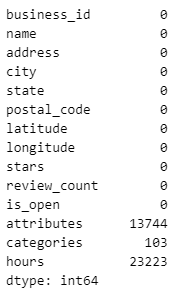
\includegraphics[width=1\columnwidth / 3]{imgs/null_count_businesses.png}
    \caption{Distribution of \texttt{null} values in \texttt{businesses}}
    \label{fig:null_count_businesses}
\end{figure}

\bigskip

This is not surprising at all because some businesses might not have specified opening hours or attributes. For $103$ businesses no category is specified. It seemed like that having one of them \texttt{null} was uncorrelated with the others being \texttt{null}, so I let MongoDB handle the missing fields.

\section{Data normalization}
In this part of the preprocessing, I dived deeper into the DataFrames to prepare them for the following shaping phase. 

First, uninteresting columns were dropped and complex JSON structures (like the one for \texttt{attributes}) flattened using \texttt{flatten()} method of \texttt{flatten\_json} library. In \texttt{elite} column there were \texttt{null} values and not coherent or repeated years (like $20$ for $2020$). 

It emerged that $44.19\%$ of total users didn't have any friends: this seemed uncorrelated with average star ratings or number of compliments received, so no rows were dropped. Also, upon having verified that $\texttt{users["friends"]} \not \subset \texttt{users["userd\_id"]}$, I have filtered out them with the method \texttt{filter\_list()}.

The same problem arose in \texttt{businesses} and \texttt{reviews} collection: there were users who have written some reviews but their \texttt{user\_id} was not in \texttt{users["user\_id"]}: I dropped them from \texttt{reviews} DataFrame. 

Luckily, $\texttt{reviews["buiness\_id"]} \subset \texttt{businesses["business\_id"]}$. 

For each business, check-ins were stored in the form of an array of dates. Pandas is not able to directly convert dates in it during reading phase, so the following was employed:

\bigskip

\begin{minted}{python}
checkins["date"] = checkins["date"].str.split(", ")
checkins["date"] = checkins["date"].apply(lambda x : pd.to_datetime(x, 
format = '%Y-%m-%d %H:%M:%S'))
\end{minted}

\bigskip

Then, to make the dates compatible with MongoDB:
\begin{minted}{python}
checkins["date"] = checkins["date"].apply(lambda x: 
date.to_pydatetime() for date in x])
\end{minted}

\section{Data shaping}
If I loaded users, businesses, reviews and check-ins in DBMS and then query the DB with \texttt{\$lookup} (the MongoDB counterpart of SQL \texttt{join}), I wouldn't have been leveraging the main feature of MongoDB that is embedding documents inside others.

The idea, here, was to embed \texttt{reviews} and \texttt{checkins} inside \texttt{businesses}. To do this, first reviews and check-ins were grouped on \texttt{business\_id} obtaining relations of the form:
$$\texttt{business\_id} \longrightarrow \texttt{[reviews for that business\_id]}$$
$$\texttt{business\_id} \longrightarrow \texttt{[checkins for that business\_id]}$$
Then, a Pandas \texttt{merge} was performed:

\bigskip

\begin{minted}{python}
businesses.merge(reviews_grouped.rename("reviews"), 
                 on = 'business_id', how = 'left')\
          .merge(checkins_grouped.rename("checkins"), 
                 on = 'business_id', how = "left")
\end{minted}

\bigskip

Finally, redundant \texttt{business\_id} column used in \texttt{merge} was removed. The resulting DataFrame (\texttt{buinesses\_merged}) was the following:

\bigskip

\begin{figure}[H]
    \centering
    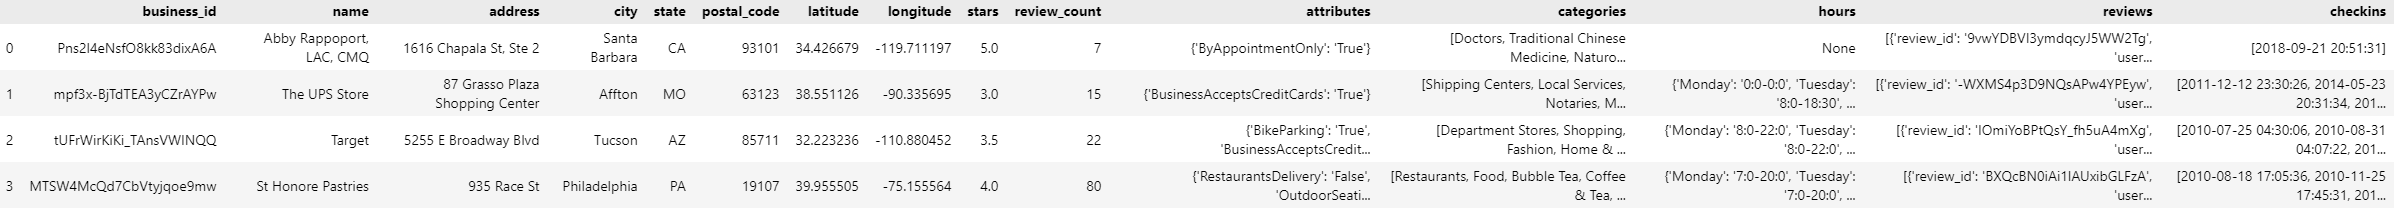
\includegraphics[width=1.1\columnwidth]{imgs/businesses_merged.png}
    \caption{DataFrame \texttt{businesses\_merged}}
    \label{fig:businesses_merged}
\end{figure}

\bigskip

Same procedure was applied for \texttt{users} and \texttt{reviews}. I started by grouping reviews, this time, on \texttt{user\_id}, then I merged each group with the \texttt{users} DataFrame and finally I dropped redundant joining attribute \texttt{user\_id} from the resulting table. The resulting DataFrame \texttt{users\_merged} is the following:

\bigskip

\begin{figure}[H]
    \centering
    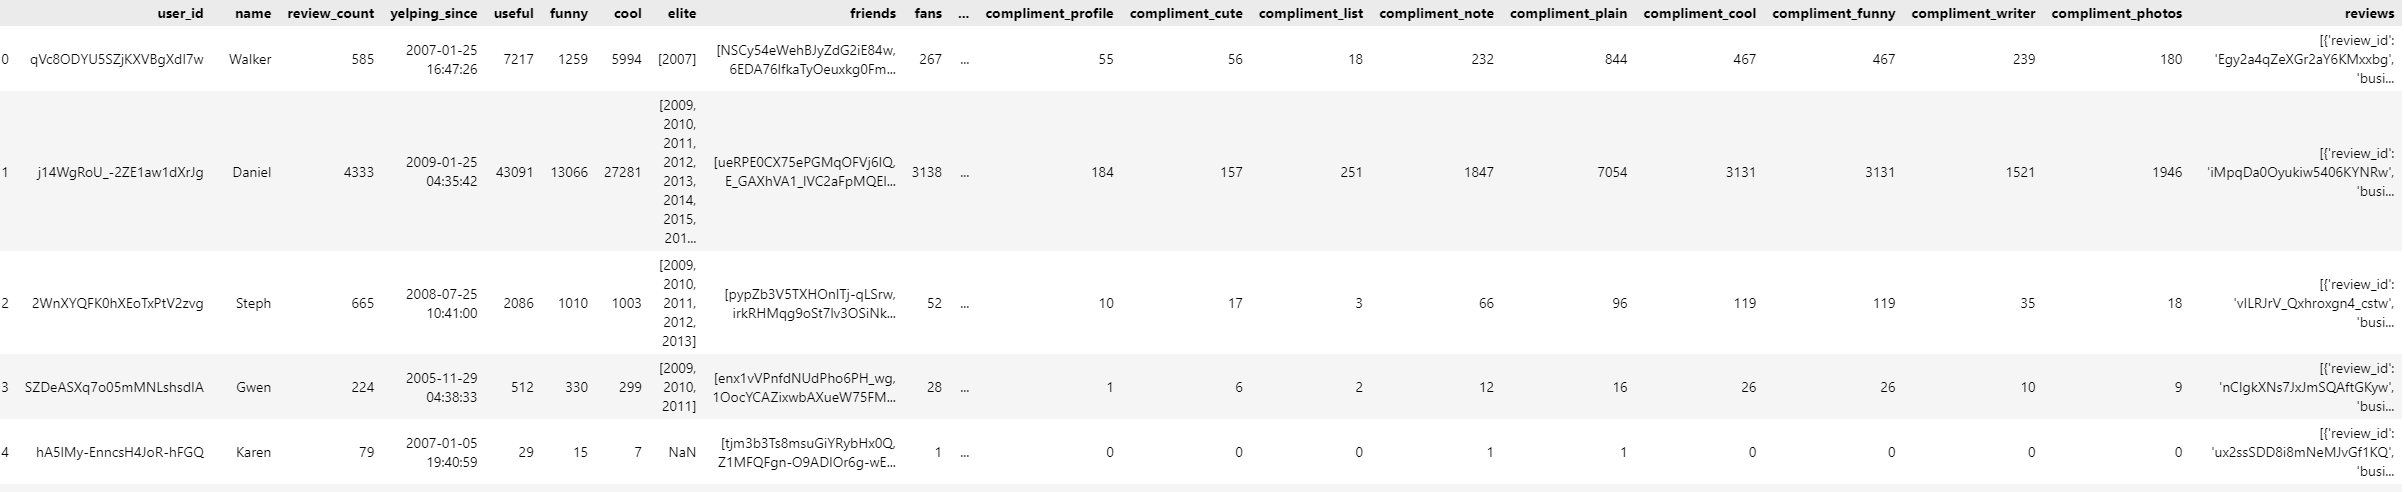
\includegraphics[width=1.1\columnwidth]{imgs/users_merged.png}
    \caption{DataFrame \texttt{users\_merged}}
    \label{fig:users_merged}
\end{figure}

\bigskip

\cleardoublepage

\chapter{Data ingestion and schema design}
This chapter focuses on the process of importing data into the database and defining its structure. It explains how the data was loaded into MongoDB and the schema design used to organize and store it effectively. By the end of the chapter, the dataset will be ready for efficient querying and analysis.

\section{Data loading}
Loading that amount of documents directly through MongoDB GUI was infeasible, so PyMongo and pre-computed Pandas DataFrames were leveraged. 

First, a connection was established with the server with the following statement: \\
\verb|client = pymongo.MongoClient("mongodb://localhost:27017/")|; then, a DB instance was created \verb|db = client["yelp"]|. 
To speed up the injection process, I employed batch loading: at each iteration a chunck (of size \texttt{batch\_size = 1000}) of original DataFrame was inserted in the DB using \texttt{db[collection\_name].insert\_many(records)}. A TQDM progress bar was displayed for each collection.

\bigskip

\begin{figure}[H]
    \centering
    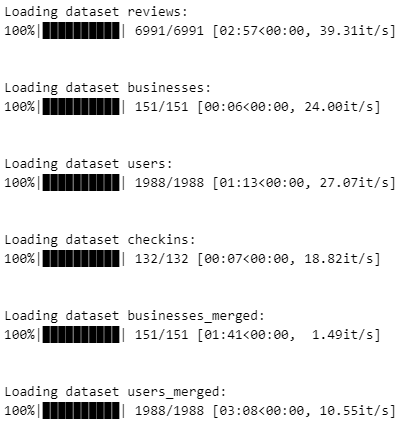
\includegraphics[width=1\columnwidth / 2]{imgs/injection_process.png}
    \caption{Loading collections in DB instance}
    \label{fig:injection_process}
\end{figure}

\bigskip

\section{Schema definition}
As the reader will surely have noticed, not only the aggregated collections but also the individual collections resulting from the analysis and cleaning of the JSON files were loaded into the database. This approach was intentional because some queries required working on single entities independently of their relationships with others.

While one might argue that this created redundancy, it was a deliberate trade-off to improve performance. By having individual collections readily available, queries that do not depend on relationships can be executed faster and more efficiently.

Individual collections have the following shape:
\begin{itemize}

\item{\texttt{businesses}}
\begin{longtable}{|p{3cm}|p{3cm}|p{10cm}|}
\hline
\textbf{Field Name} & \textbf{Type} & \textbf{Description} \\ \hline
\texttt{business\_id} & \texttt{string} & Unique identifier for the business (22 characters). \\ \hline
\texttt{name} & \texttt{string} & The name of the business. \\ \hline
\texttt{address} & \texttt{string} & Full address of the business. \\ \hline
\texttt{city} & \texttt{string} & City where the business is located. \\ \hline
\texttt{state} & \texttt{string} & State code (2 characters). \\ \hline
\texttt{postal\_code} & \texttt{string} & Postal code of the business. \\ \hline
\texttt{latitude} & \texttt{float} & Latitude of the business location. \\ \hline
\texttt{longitude} & \texttt{float} & Longitude of the business location. \\ \hline
\texttt{stars} & \texttt{float} & Star rating, rounded to half-stars. \\ \hline
\texttt{review\_count} & \texttt{integer} & Number of reviews for the business. \\ \hline
\texttt{is\_open} & \texttt{integer} & Indicates whether the business is open (1 for open, 0 for closed). \\ \hline
\texttt{attributes} & \texttt{dict} & Key-value pairs of business attributes (e.g., parking availability). \\ \hline
\texttt{categories} & \texttt{array[string]} & Array of strings representing business categories. \\ \hline
\texttt{hours} & \texttt{dict} & Key-value pairs of operating hours by day. \\ \hline
\caption{\texttt{businesses} collection}
\end{longtable}

\item{\texttt{reviews}}
\begin{longtable}{|p{3cm}|p{3cm}|p{10cm}|}
\hline
\textbf{Field Name} & \textbf{Type} & \textbf{Description} \\ \hline
\texttt{review\_id} & \texttt{string} & Unique identifier for the review (22 characters). \\ \hline
\texttt{user\_id} & \texttt{string} & Unique identifier for the user who wrote the review. \\ \hline
\texttt{business\_id} & \texttt{string} & Unique identifier for the business the review is written for. \\ \hline
\texttt{stars} & \texttt{integer} & Star rating given in the review. \\ \hline
\texttt{date} & \texttt{DateTime} & Date of the review (format: YYYY-MM-DD HH:MM:SS). \\ \hline
\texttt{text} & \texttt{string} & The text of the review. \\ \hline
\texttt{useful} & \texttt{integer} & Number of useful votes received by the review. \\ \hline
\texttt{funny} & \texttt{integer} & Number of funny votes received by the review. \\ \hline
\texttt{cool} & \texttt{integer} & Number of cool votes received by the review. \\ \hline
\caption{\texttt{reviews} collection}
\end{longtable}

\item{\texttt{users}}
\begin{longtable}{|p{3cm}|p{3.5cm}|p{10cm}|}
\hline
\textbf{Field Name} & \textbf{Type} & \textbf{Description} \\ \hline
\texttt{user\_id} & \texttt{string} & Unique identifier for the user (22 characters). \\ \hline
\texttt{name} & \texttt{string} & User's first name. \\ \hline
\texttt{review\_count} & \texttt{integer} & Number of reviews written by the user. \\ \hline
\texttt{yelping\_since} & \texttt{DateTime} & Date the user joined Yelp (format: YYYY-MM-DD HH:MM:SS).\\ \hline
\texttt{friends} & \texttt{array[string]} & Array of user IDs representing the user's friends. \\ \hline
\texttt{useful} & \texttt{integer} & Number of useful votes sent by the user. \\ \hline
\texttt{funny} & \texttt{integer} & Number of funny votes sent by the user. \\ \hline
\texttt{cool} & \texttt{integer} & Number of cool votes sent by the user. \\ \hline
\texttt{fans} & \texttt{integer} & Number of fans the user has. \\ \hline
\texttt{elite} & \texttt{array[int]} & Years the user was marked as elite. \\ \hline
\texttt{average\_stars} & \texttt{float} & User's average star rating across all reviews. \\ \hline
\caption{\texttt{users} collection}
\end{longtable}

\item{\texttt{checkins}}
\begin{longtable}{|p{3cm}|p{3.5cm}|p{10cm}|}
\hline
\textbf{Field Name} & \textbf{Type} & \textbf{Description} \\ \hline
\texttt{business\_id} & \texttt{string} & Unique identifier for the business (22 characters). \\ \hline
\texttt{date} & \texttt{array[DateTime]} & Comma-separated list of timestamps (format: YYYY-MM-DD HH:MM:SS). \\ \hline
\caption{\texttt{checkins} collection}
\end{longtable}

\end{itemize}

The structure of \texttt{businesses\_merged} and \texttt{users\_merged} is not shown because the reader can easily infer it from the previously presented tables.

\section{Indexing}
MongoDB assigns by default to each object a unique ID. With such a large amount of data, it is fundamental to define custom indices to keep good queries performance. I did it directly in the notebook using PyMongo \texttt{create\_index()} method:

\bigskip

\begin{minted}{python}
#For "businesses", we need only "business_id" as index
db["businesses"].create_index(["business_id"], unique = True)

#For "users", we need only "user_id" as index
db["users"].create_index(["user_id"], unique = True)

#For "checkins", we need only "business_id" as index
db["checkins"].create_index(["business_id"], unique = True)

#For "reviews", we need "business_id", "user_id" and "review_id" as index
db["reviews"].create_index(["business_id"])
db["reviews"].create_index(["user_id"])
db["reviews"].create_index(["review_id"], unique = True)

#For "businesses_merged", we need "business_id" as index
db["businesses_merged"].create_index(["business_id"], unique = True)

#For "users_merged", we need "user_id" as index
db["users_merged"].create_index(["user_id"], unique = True)
\end{minted}

\bigskip

where \texttt{unique = True} parameter tells MongoDB that index values are unique (it is not the case of \texttt{user\_id} in \texttt{reviews} because one user might appear in more than one document). 

\cleardoublepage

\chapter{Sentiment analysis}
In this chapter, the reader is presented with the preprocessing work done for sentiment analysis phase (extra). 

\section{Sentiment analysis model}
\label{sent_model}
The model used for performing sentiment analysis is \texttt{distilbert-base-uncased-\\finetuned-sst-2-english} that is a lightweight, fine-tuned version of DistilBERT. It has been derived from the \texttt{distilbert-base-uncased} architecture by fine-tuning it on the Stanford Sentiment Treebank (SST-2) dataset. It classifies text into positive or negative categories. 

I chose it because it is one of the most used models for social media monitoring, customer feedback analysis or product review assessments and it is able to achieve high accuracy despite its compact size.
Furthermore, the fine-tuning process on SST-2 enhances the model's capability to identify nuanced emotional expressions, such as irony or strong sentiments. 

It's said to be "uncased" because it treats upper / lower case letters in the same manner.

As all the other transformers architectures, the model employs self-attention mechanisms to process input sequences and capture context.

Once having installed \textit{PyTorch} and \texttt{transformers} module from \textit{HuggingFace}, it's API is very simple to use:

\bigskip

\begin{minted}{python}
from transformers import pipeline

classifier = pipeline("sentiment-analysis", 
                      model = """distilbert-base-uncased-finetuned-sst-
                      2-english""")

text = "This product works amazingly well!"
result = classifier(text)
print(result)
\end{minted}

\bigskip

The output is: 

\texttt{Device set to use cuda:0}

\verb|[{'label': 'POSITIVE', 'score': 0.9998623132705688}]|

\section{Objective}
Sentiment analysis was not the first thing done after the dataset was loaded. The majority of the queries were performed, and, upon having analysed their results, the idea of applying sentiment analysis came up. 

The ultimate goal was to bridge the gap between quantitative (stars) and qualitative (text) feedback to provide insights into user reviews. For example, by exploring the relationship between review sentiment and star ratings, one could assess how well the sentiment in text aligns with the corresponding star rating; cases where positive sentiment accompanies a low star rating, or vice versa, might provide insights of biases into user behaviour. Or, by segmenting users based on the typical sentiment of their reviews, one could assist businesses in better interpreting customer feedback. 

\section{Methodology}
In this section, I present how sentiment analysis pipeline was integrated with MongoDB existing collections. 

\subsection{Data extraction}
Firstly, data had to be retrieved and put in a DataFrame. A simple MongoDB query was written and executed:

\bigskip

\begin{minted}{python}
client = pymongo.MongoClient("mongodb://localhost:27017/")
db = client["yelp"]

reviews = db["reviews"].find({}, {
    "review_id" : 1,
    "text" : 1
})

reviews = pd.DataFrame(reviews)
reviews = reviews.set_index("review_id")
reviews
\end{minted}

\bigskip

Note that \texttt{\_id} column wasn't kept, but only \texttt{review\_id} column because as mentioned in previous chapter, I created an index on it.  

\subsection{Model usage}
The main class is \texttt{SentimentAnalyzer}.

First, text was preprocessed: each review text was mapped into numerical tokens that the model is able to understand. Naturally, text varies in length, so padding and truncation were used to ensure consistent input lengths:

\begin{verbatim}
tokenizer(texts, 
         max_length = self.max_length, 
         padding = True, 
         truncation = True, 
         return_tensors = "pt")
\end{verbatim}

To optimize memory usage, the model operated in half-precision mode when using GPU:
\begin{verbatim}
if self.device == "cuda":
    self.model = self.model.half()
\end{verbatim}

Dataset consisted of about $7$ million reviews and all of them needed to be processed to have good results, so batching and chunking strategies were applied:
\begin{itemize}
    \item Chunks: large portions of the dataset (e.g. $10,000$ reviews) that were loaded into memory and stored in CSV file at once;
    \item (Mini-) Batches: smaller groups (e.g. $512$ reviews) within each chunk that were processed together by the GPU.
\end{itemize}

This was implemented as nested loops:
\begin{verbatim}
for start_idx in range(0, total_rows, chunk_size):
    chunk_df = df.iloc[start_idx : end_idx]
    
    for batch_start in range(0, len(chunk_df), self.batch_size):
        batch_df = chunk_df.iloc[batch_start : batch_end]
\end{verbatim}

Once having defined the \texttt{analyzer}, I used it:

\begin{minted}{python}
analyzer = SentimentAnalyzer("""distilbert-base-uncased-finetuned
                             -sst-2-english""", 
                             batch_size = 512, max_length = 256)

analyzer.process_reviews(reviews, 
                         "sentiment_results.csv", 10000)
\end{minted}

where \texttt{max\_length} is the maximum number of tokens in which text was split up by the tokenizer. The model was trained and fine-tuned with sequences of maximum length of $512$, so all values below should be fine. By inspecting the distribution of number of tokens per reviews, $256$ seemed a good compromise between performance and expressiveness:

\bigskip

\begin{figure}[H]
    \centering
    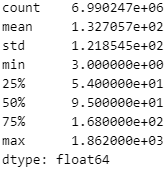
\includegraphics[width=1\columnwidth / 4]{imgs/num_tokens.png}
    \caption{Distribution of number of tokens}
    \label{fig:token_distr}
\end{figure}

\bigskip

The resulting CSV file contained on each line a triplet: \texttt{(review\_id, sentiment, \\score)}

\subsection{Collections update}
Both \texttt{reviews}, \texttt{users\_merged} and \texttt{businesses\_merged} had to be updated by adding the new fields. To do this in an efficient way, I converted the resulting DataFrame to a dictionary and then, I leveraged  \texttt{pyMongo.updateOne()} along with \texttt{bulk\_write()}. I chose to use \texttt{bulk\_write()} to reduce as much as possible the number of transactions; namely, this method is able to perform multiple write operations (inserts, updates or deletes) in a single request to the database. 

Different collections required different update strategies:
\begin{itemize}
    \item In \texttt{reviews} collection, each document contains a single review and an index was present on \texttt{review\_id}, so it was sufficient to filter on it:
    \bigskip
    
    \begin{minted}{python}
db["reviews"].bulk_write([
    pymongo.UpdateOne({
          "review_id" : review_id
      },
      {
          "$set" : data
      })
      for review_id, data in batch_items
])
    \end{minted}
    
    \bigskip

    \item In \texttt{businesses\_merged}, each \texttt{business\_id} mapped a set of reviews. So, I needed a dictionary $\texttt{review\_id} \longrightarrow \texttt{business\_id}$ \\and an additional index on \texttt{reviews.review\_id} that is sparse because some documents might not have \texttt{reviews} sub-collection:
    \bigskip
    
    \begin{minted}{python}
db["businesses_merged"].create_index(["reviews.review_id"], 
                                     unique = True, sparse = True)
    \end{minted}
    
    \bigskip
    In the filter condition of \texttt{updateOpne()}, the review is located by looking at \texttt{business\_id} and \texttt{reviews.review\_id}. Then, in \texttt{\$set}, \texttt{\$} is used to catch the matching document(s) to insert the new fields into.
    \bigskip
    
    \begin{minted}{python}
        db["businesses_merged"].bulk_write([
              pymongo.UpdateOne({ 
                    "business_id" :review_to_business_map[review_id],
                    "reviews.review_id" : review_id 
                },
                {
                    "$set" : {
                        "reviews.$.sentiment" : data["sentiment"],
                        "reviews.$.confidence" : data["confidence"]  
                    }
                })
                for review_id, data in batch_items
      ])
        
    \end{minted}
    
    \bigskip

    \item In \texttt{users\_merged} same challenges of \texttt{businesses\_merged} were faced. I repeated what is shown in the previous case.
\end{itemize}

\cleardoublepage

\chapter{Queries}
In this chapter, the user is presented with the queries performed in MongoDB. All of them were executed within a Jupyter Notebook connected to MongoDB instance using \texttt{PyMongo}. Some interesting results were visualized using \texttt{matplotlib.pyplot}, \texttt{seaborn} libraries.

\section{Query 1: how many businesses and reviews for each category?}

The purpose of this query was to count the total number of businesses and reviews for each category of businesses.

\bigskip
    
\begin{lstlisting}[style=mongodb]
db["businesses_merged"].aggregate([
    {
        "$project" : {
            "categories" : 1,
            "reviews" : 1,
            "business_id" : 1
        }
      },
    {
        "$unwind" : "$categories"
    },
    {
        "$unwind" : "$reviews"
    },
    {
        "$group" : {
            "_id" : "$categories",
            "num_reviews" : {
                "$sum" : 1
            },
            "ids" : {
                "$addToSet" : "$business_id"
            }
        }
    },
    {
        "$project" : {
            "_id" : 0,
            "category" : "$_id",
            "num_businesses" : {
              "$size" : "$ids"
            },
            "num_reviews" : 1
        }
    },
    {
        "$sort" : {
            "num_businesses" : -1,
            "num_reviews" : -1
        }
    }
])
 
\end{lstlisting}

\bigskip

This query is a clear example of applying NoSQL principles (in particular, document embedding), as it uses documents with sub-collections and deconstructs nested arrays using \texttt{\$unwind}. In contrast, the following query is more aligned with traditional SQL principles, as it relies on \texttt{\$lookup} to join collections:

\bigskip
    
\begin{lstlisting}[style=mongodb]
db["reviews"].aggregate([
    {
        "$lookup" : { 
            "from" : "businesses",
            "let" : { 
                "id" : "$business_id"
            },
            "pipeline" : [{
                            "$match" : { 
                                "$expr" : { 
                                    "$eq" : ["$business_id", "$$id"]
                                }                          
                            }   
                         }],
            "as" : "business" 
        }
    },
    {
        "$unwind" : "$business"
    },
    {
        "$unwind" : "$business.categories"
    },
    {
        "$group" : {
            "_id" : "$business.categories",
            "num_reviews" : {
                "$sum" : 1
            },
            "ids" : {
                "$addToSet" : "$business.business_id"
            }
        }
    },
    {
        "$project" : {
            "_id" : 0,
            "category" : "$_id",
            "num_businesses" : {
                "$size" : "$ids"
            },
            "num_reviews" : 1
        }
    },
    {
        "$sort" : {
            "num_businesses" : -1,
            "num_reviews" : -1
        }
    }
])
 
\end{lstlisting}

\bigskip

In the notebook, under \texttt{Query 1} subsection, the reader will find another version of this query (here not shown for the sake of shortness) that combines MongoDB and Pandas.

\bigskip

Although taking different times, all the queries produce the same resulting DataFrame:

\bigskip

\begin{figure}[H]
    \centering
    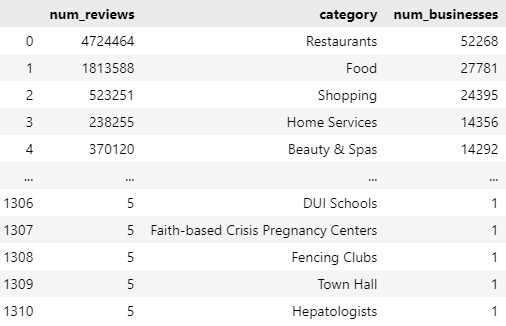
\includegraphics[width=2\columnwidth / 3]{imgs/businesses_and_reviews_per_category.png}
    \caption{Number businesses and reviews per category}
    \label{fig:num_businesses_and_reviews_per_category}
\end{figure}

\bigskip

The result show that there are $1,311$ different categories. \textit{"Restaurants"} and \textit{"Food"} categories dominate in terms of both the number of reviews ($4.7\text{M}$ and $1.8\text{M}$, respectively) and businesses ($52,268$ and $27,781$), making them highly competitive sectors. 

On the other hand, categories like \textit{"Home Services"} ($238,255$ reviews, $14,356$ businesses) and \textit{"Beauty \& Spas"} ($370,120$ reviews, $14,292$ businesses) are subject to moderate competition with still a quite significant demand.

A possible conclusion is that, even if the first categories may still offer growth opportunities, new investments would probably have more success in the others. For niche opportunities, categories with fewer businesses but steady demand, such as "Shopping", could also be worth exploring. 

\section{Query 2: for each category, find the most polarizing business}
A business is said to be \textit{"polarizing"} if it is one with high variance in star rating. The objective of this query was to identify, for each category, the most polarizing business.

For this query, \texttt{\$stdDevPop} was employed.

\bigskip

\begin{lstlisting}[style=mongodb]
db["reviews"].aggregate([
    {
        "$project" : {
            "business_id" : 1,
            "categories" : 1,
            "reviews.stars" : 1,
            "name" : 1
        }
    },
    {
        "$unwind" : "$categories"
    },
    {
        "$unwind" : "$reviews"
    },                                      
    { 
        "$group" : {
            "_id" : {
                "r_id" : "$business_id",
                "category" : "$categories"
            },
            "name" : {
                "$first" : "$name"
            },
            "avg_stars" : {
                "$avg": "$reviews.stars"
            },
            "variance" : {
                "$stdDevPop": "$reviews.stars" 
            },
            "num_reviews" : {
                "$sum" : 1
            } 
        }
    },
    {
        "$sort" : {
            "category" : 1,
            "variance" : -1
        }
    },
    {
        "$group" : {
            "_id" : "$_id.category",
            "name" : {
                "$first" : "$name"
            },
            "variance" : {
                "$first" : "$variance"
            },
            "avg_stars" : {
                "$first": "$avg_stars"
            },
            "num_reviews" : {
                "$first": "$num_reviews"
            }
        }
    },
    {
        "$project" : {
            "_id" : 0,
            "category" : "$_id",
            "name" : 1,
            "avg_stars" : 1,
            "num_reviews" : 1,
            "variance" : 1,
        }
    },
    {
        "$sort" : {
            "variance" : -1
        }
    }
])
\end{lstlisting}

\bigskip

For some categories ("Medical Centers", "Restaurants", "Pets", "Optometrists", "Aquarium Services", "Somali"), number of reviews along with average and variance were plotted:

\bigskip

\begin{figure}[H]
    \centering
    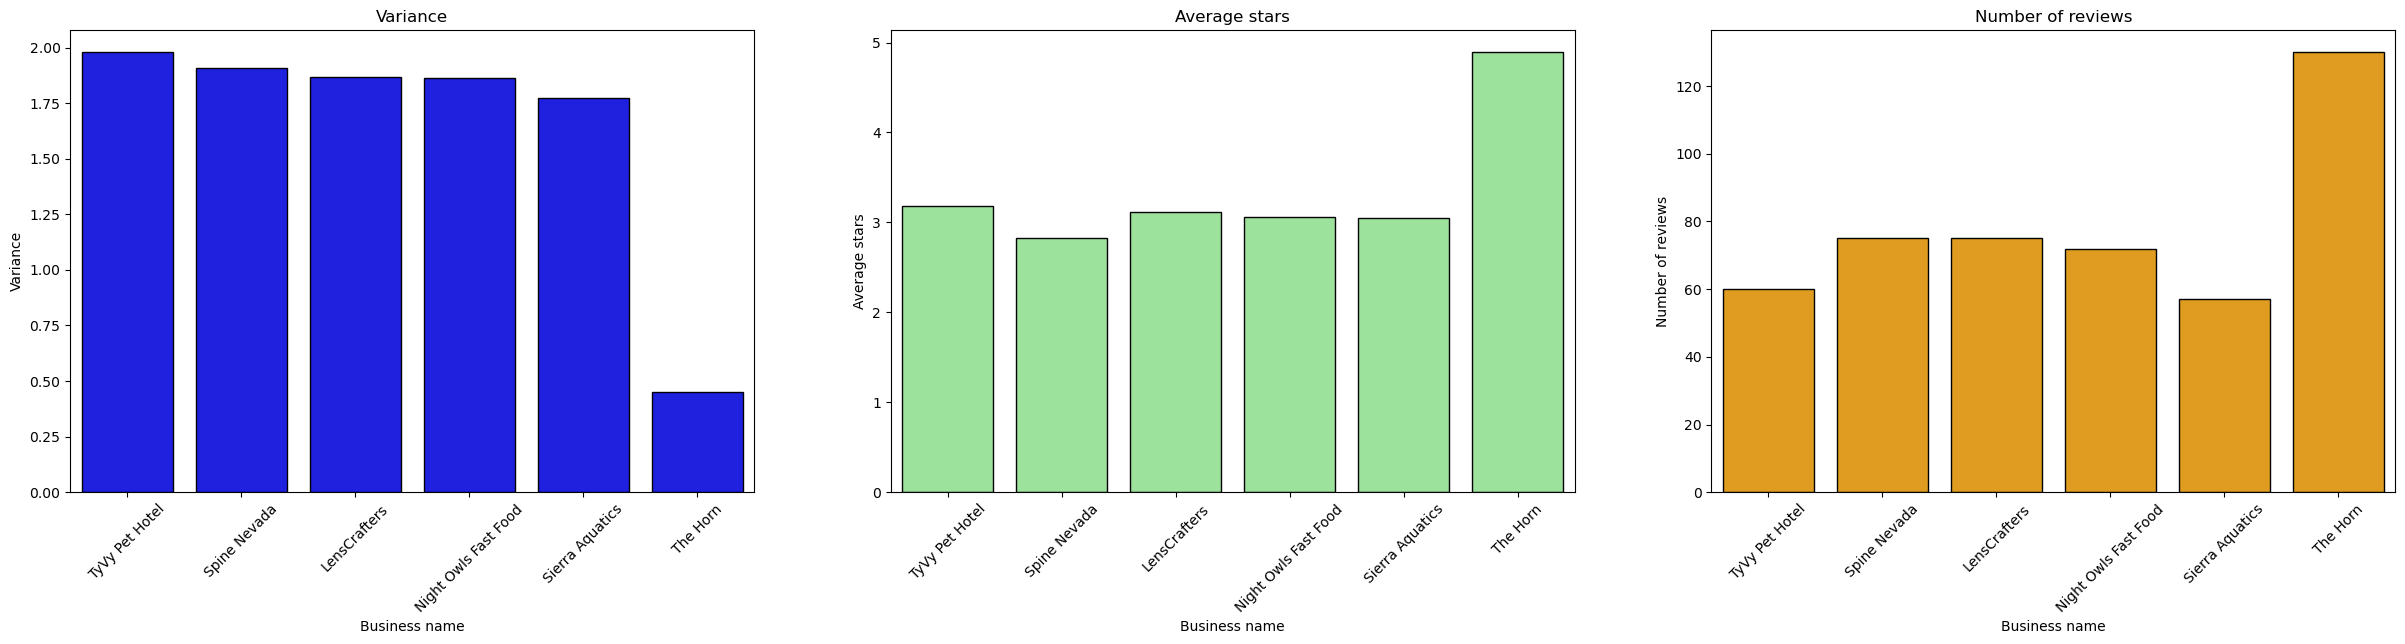
\includegraphics[width=\columnwidth]{imgs/most_polarizing_businesses.png}
    \caption{Most polarizing businesses for some categories}
    \label{fig:most_polarizing_businesses}
\end{figure}

\bigskip

The entire DataFrame is the following:

\bigskip

\begin{figure}[H]
    \centering
    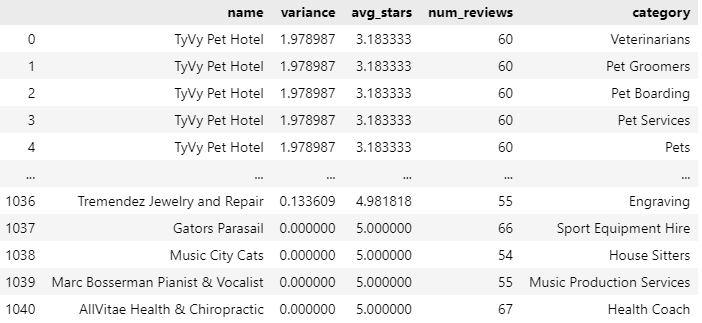
\includegraphics[width=\columnwidth]{imgs/most_polarizing_businesses_table.png}
    \caption{DataFrame of most polarizing businesses for some categories}
    \label{fig:most_polarizing_businesses_table}
\end{figure}

\bigskip

In the query, only businesses with at least 50 reviews were selected to minimize potential bias in the variance. Notably, the \textit{"restaurants"} category stands out as one of those with the highest variance: this is reasonable because restaurants cater to a wide range of customer preferences that leads to greater variability in reviews. Also, the categories \textit{"pets"} and \textit{"medical centers"} show high variance. For the first, this could be due to the emotional weight of customers experience with pet services. For the latter, it might come from from the critical nature of healthcare services, where individual experiences can vary dramatically based on the quality of care, wait times, or outcomes.

Note that the number of reviews and the average star ratings are relatively consistent across categories: this is important because it means that a uniform sample was chosen. 

\section{Query 3: find in which city a chain of businesses performs the best}
A chain of businesses is a set of \texttt{business\_id} with the same \texttt{name} but different \texttt{city}. The goal of this query was to discover in which city a chain of businesses performs the best. Note that in a city there could be more than one \texttt{business\_id} with the same name.

In the first step of the query, all the necessary documents were retrieved using MongoDB:
\begin{itemize}
    \item \texttt{more\_than\_one\_city}: all chains of businesses were collected.

\bigskip

\begin{lstlisting}[style=mongodb]
db["businesses"].aggregate([{
        "$group" : {
            "_id" : {
                "name" : "$name", 
            },
            "cities" : {
                "$addToSet" : "$city"
            }
        }
    },
    {
        "$match" : {
            "$expr" : {
                "$gt" : [{"$size" : "$cities"}, 1]
            }
        }
    },
    {
        "$project" : {
            "_id" : 0,
            "name" : "$_id.name",
            "num_cities" : {"$size" : "$cities"}
        }
    }
])
\end{lstlisting}

\bigskip

\item \texttt{ratings}: for each business name and each city, the average rating was computed.

\bigskip

\begin{lstlisting}[style=mongodb]
db["businesses_merged"].aggregate([{
    "$project" : {
        "name" : 1,
        "city" : 1,
        "reviews.stars" : 1,
    }
},
{
        "$unwind" : "$reviews" 
    },
    {
        "$group" : {
            "_id" : {
                "name" : "$name", 
                "city" : "$city" 
            },
            "avg_stars" : {
                "$avg" : "$reviews.stars" 
            }
        }
    },
    {
        "$project" : {
            "_id" : 0,
            "name" : "$_id.name",
            "city" : "$_id.city",
            "avg_stars" : 1
        }
    },
    {
        "$sort" : {
            "name" : 1,
            "avg_stars" : -1
        }
    },
    {
        "$group" : {
            "_id" : "$name",
            "city" : { 
                "$first" : "$city"
            },
            "avg_stars" : {
                "$first" : "$avg_stars"
            }
        }
    },
    {
        "$project" : {
            "_id" : 0,
            "name" : "$_id",
            "city" : 1,
            "avg_stars" : 1
        }
    }
])
\end{lstlisting}

\bigskip
\end{itemize}

In the second step, the intersection between \texttt{more\_than\_one\_city} and \texttt{ratings} was computed using Pandas:

\bigskip 

\begin{minted}{python}
df = pd.DataFrame(ratings)
df = df[df["name"].isin(more_than_one_city["name"])]
\end{minted}

\bigskip

I opted for a composite query because computing and intersecting \texttt{more\_than\_one\_city} and \texttt{ratings} in a single query wasn't trivial (it could be done, but it would require the usage of \texttt{\$facet}).

The results are summarized in the following DataFrame:

\bigskip

\begin{figure}[H]
    \centering
    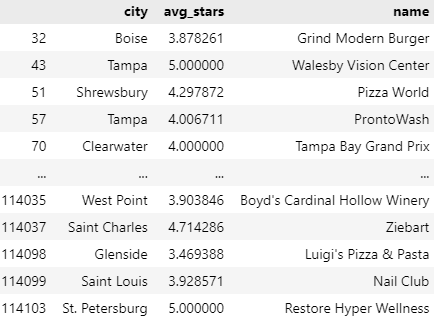
\includegraphics[width=2\columnwidth / 3]{imgs/query_4_table.png}
    \caption{Best city for chains of businesses}
    \label{fig:query_4}
\end{figure}

\bigskip

\section{Query 4: establish whether local competitions influences average and variance review stars}
Two businesses $\texttt{b}_1$ and $\texttt{b}_2$ are said to be competitors if they share at least one category (i.e. $\texttt{b}_1\texttt{.category} \cap \texttt{b}_2\texttt{.category} \neq \{\emptyset\}$ and they work in the same city (i.e. $\texttt{b}_1\texttt{.city} = \texttt{b}_2\texttt{.city}$). 

With this query, I studied whether there was a relation between the average (variance) of reviews' stars and the number of competitors for the most widespread businesses. 

As done in the previous query, I proceeded with a two-steps query. In the first one, all relevant documents were shaped and retrieved:
\begin{itemize}
    \item \texttt{competitors}: for each \texttt{name} and \texttt{city}, the number of competitors was computed. 

\bigskip

\begin{lstlisting}[style=mongodb]
db["businesses"].aggregate([{
        "$unwind" : "$categories"
    },
    {
        "$group" : {
            "_id" : {
                "city" :"$city",
                "category" : "$categories"
            },
            "businesses_names" : {
                "$addToSet" : "$name"
            }
        }
    },
    {
        "$addFields" : {
            "businesses_names_copy" : "$businesses_names"
        }
    },
    {
        "$unwind" : "$businesses_names"
    },
    {
        "$group" : {
            "_id" : {
                "name" : "$businesses_names",
                "city" : "$_id.city"
            },
            "possible_competitors" : {
                "$addToSet" : "$businesses_names_copy"
            }
        }
    },
    {
        "$project" : { 
            "_id" : 1,
            "possible_competitors" : {
                "$filter" : {
                    "input" : "$possible_competitors",
                    "as" : "pc",
                    "cond" : {
                        "$ne" : ["$$pc", "$_id.name"]
                    }
                }
            }
        }
    },
    {
        "$addFields" : {
            "num_competitors" : {
                "$size" : "$possible_competitors"
            }
        }
    },
    {
        "$project" : {
            "_id" : 0,
            "city" : "$_id.city",
            "name" : "$_id.name",
            "num_competitors" : 1
        }
    }
])
\end{lstlisting}

\bigskip

The reasoning behind this query is quite complex; to fully understand it, it's better to outline the structure oof documents after each stage:

\begin{enumerate}
\item In the \texttt{\$unwind} stage documents with multiple categories were split, creating separate documents for each category.

\item Documents were grouped by \texttt{(city, category)} pairs using \texttt{\$group} and, for each group, the unique business names were collected into \texttt{businesses\_names}.

\item A copy of \texttt{businesses\_names} was created as \texttt{businesses\_names\_copy} for later reference.

\item The \texttt{businesses\_names} array was unwound: in each document a certain \texttt{(busi-\\ness\_name, category)} is associated with all the competitors \texttt{business\_name} for that category.

\item Then, documents were regrouped by \texttt{(name, city)}, collecting all businesses that share any category  from \texttt{businesses\_names\_copy} arrays (i.e. potential competitors).

\item With \texttt{\$project} and \texttt{\$filter}, each business was removed from its own list of competitors.

\item Number of competitors for each business was computed using \texttt{\$size}.

\item Lastly, the output was formatted to show \texttt{city}, \texttt{name}, and \texttt{num\_competitors} for each business.

\end{enumerate}

\item \texttt{ratings}: for each business, average and standard deviation of reviews' stars were computed. 

\bigskip

\begin{lstlisting}[style=mongodb]
db["businesses_merged"].aggregate([
    {
        "$unwind" : "$reviews" 
    },
    {
        "$group" : {
            "_id" : {
                "name" : "$name", 
                "city" : "$city" 
            },
            "avg_stars" : {
                "$avg" : "$reviews.stars" 
            },
            "star_variance" : {
                "$stdDevPop" : "$reviews.stars"
            }

        }
    },
    {
        "$project" : {
            "_id" : 0,
            "name" : "$_id.name",
            "city" : "$_id.city",
            "avg_stars" : 1,
            "star_variance" : 1
        }
    }
])

\end{lstlisting}

\bigskip

\end{itemize}

In the second step of the query, the two resulting DataFrames were merged using Pandas:

\bigskip 

\begin{minted}{python}
ratings_df = pd.DataFrame(ratings)
competitors_df = pd.DataFrame(competitors)
df = pd.merge(ratings_df, competitors_df, 
              left_on = ["name", "city"], right_on = ["name", "city"])
\end{minted}

\bigskip

Some results:
\bigskip

\begin{figure}[H]
    \centering
    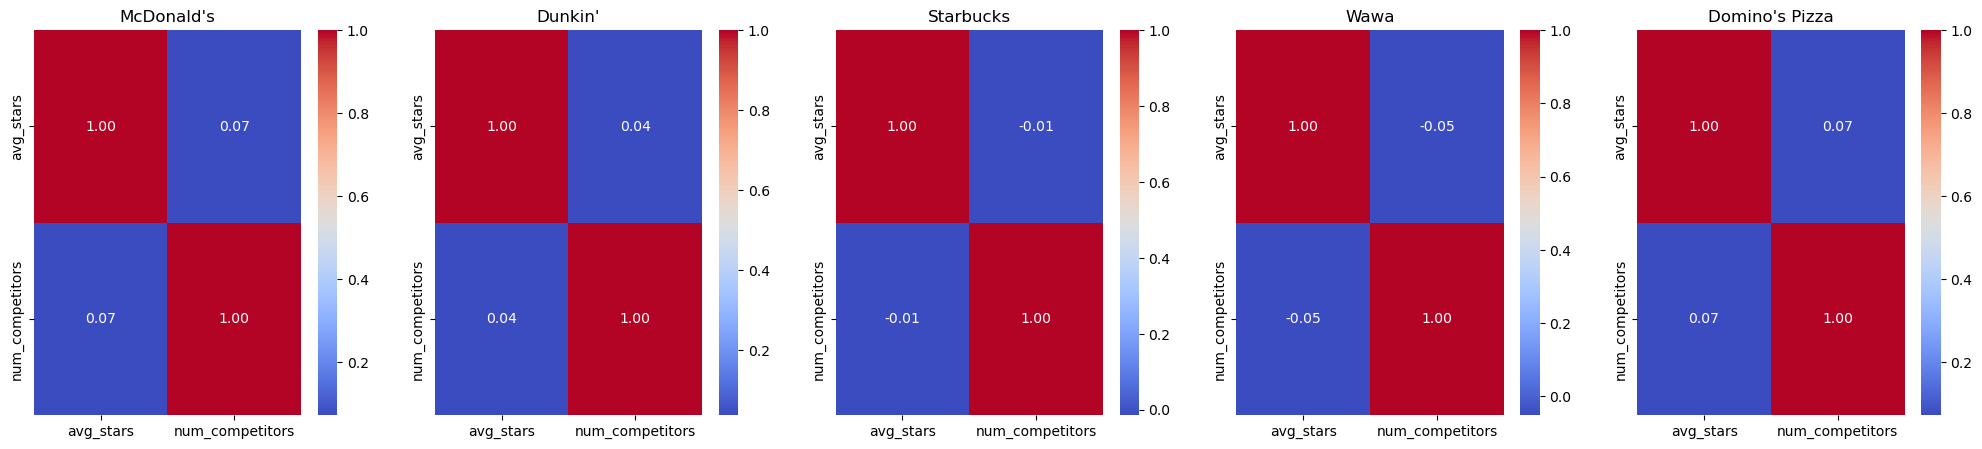
\includegraphics[width=\columnwidth]{imgs/query_4b.png}
    \caption{Average - variance vs competition for $1$st to $5$th most widespread businesses}
    \label{fig:query_4b}
\end{figure}

\bigskip

\begin{figure}[H]
    \centering
    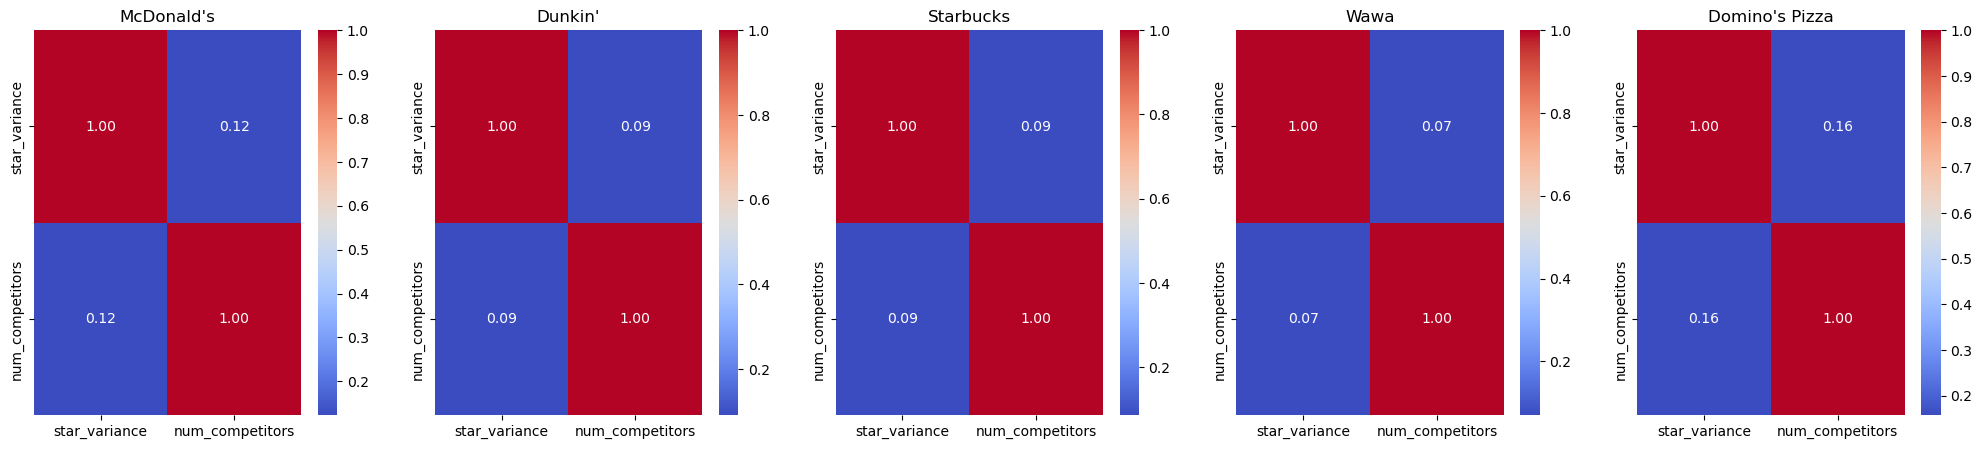
\includegraphics[width=\columnwidth]{imgs/query_4e.png}
    \caption{Variance vs competition for $1$st to $5$th most widespread businesses}
    \label{fig:query_4e}
\end{figure}

\bigskip

This results reveal mixed trends. For instance, \textit{Wawa} in Souderton has a high average rating ($4.19$) with $8$ competitors, while \textit{Domino's Pizza} in Normandy and \textit{McDonald's} in Lawrence, with fewer competitors ($3$ and $5$, respectively), exhibit much lower ratings ($1.56$ and $1.72$). 

Further analysis was executed on the $50$th to $55$th most widespread businesses and it confirmed the complexity. \textit{Waffle House} in Tampa, despite $10$ competitors, maintains a strong average rating ($3.57$), while \textit{Walmart} in Exton has $6$ competitors and is rated $1.87$. 

The star variance also varies widely, For example, \textit{Dairy Queen Grill \& Chill} in Spring Hill shows high variance ($1.77$), whereas \textit{Waffle House} in Lawrence has a more consistent satisfaction level ($1.23$).

I concluded that competition may influence ratings, but this is not an universal rule because the relationship is shaped, also, by local factors and customer expectations.

\section{Query 5: are day and night reviews biased?}
The aim of this query was to investigate whether there was a discrepancy in the reviews of the day and night for each user. Such discrepancy was estimated using average star rating.

\bigskip

\begin{lstlisting}[style = mongodb]
db["reviews"].aggregate([{
        "$project" : {
            "user_id" : 1,
            "date" : 1,
            "stars" : 1
        }
    },
    {
        "$addFields" : {
            "reviewHour" : {
                "$hour": "$date"
            }
        }
    },
    {
        "$addFields" : { 
            "is_night" : {
                "$or" : [
                    {"$gte": ["$reviewHour", 22]}, 
                    {"$lt": ["$reviewHour", 5]}
                ]
            }
        }
    },
    { 
        "$group" : {
            "_id" : "$user_id",
            "num_night_reviews" : {
                "$sum" : {
                    "$cond" : ["$is_night", 1, 0] 
                }
            },
            "num_day_reviews" : {
                "$sum" : {
                    "$cond" : ["$is_night", 0, 1]
                }
            },
            "avg_night_ratings" : {
                "$avg" : {
                    "$cond" : ["$is_night", "$stars", None] 
                } 
            },
            "avg_day_ratings" : {
                "$avg" : {
                    "$cond" : ["$is_night", None, "$stars"]
                }
            }
        }
    },
    { 
        "$match": {
            "num_night_reviews" : {
                "$gte": 5
            },
            "num_day_reviews" : {
                "$gte": 5
            },
        }
    },
    { 
        "$project" : {
            "_id": 0,
            "user_id": "$_id",
            "num_night_reviews": 1,
            "num_day_reviews": 1,
            "avg_night_ratings": 1,
            "avg_day_ratings": 1
        }
    }
])
\end{lstlisting}

\bigskip

In the notebook, under \texttt{Query 5} subsection, the reader will find another version of this query (here not shown for the sake of shortness) that combines MongoDB and Pandas.

Some results:

\bigskip

\begin{figure}[H]
    \centering
    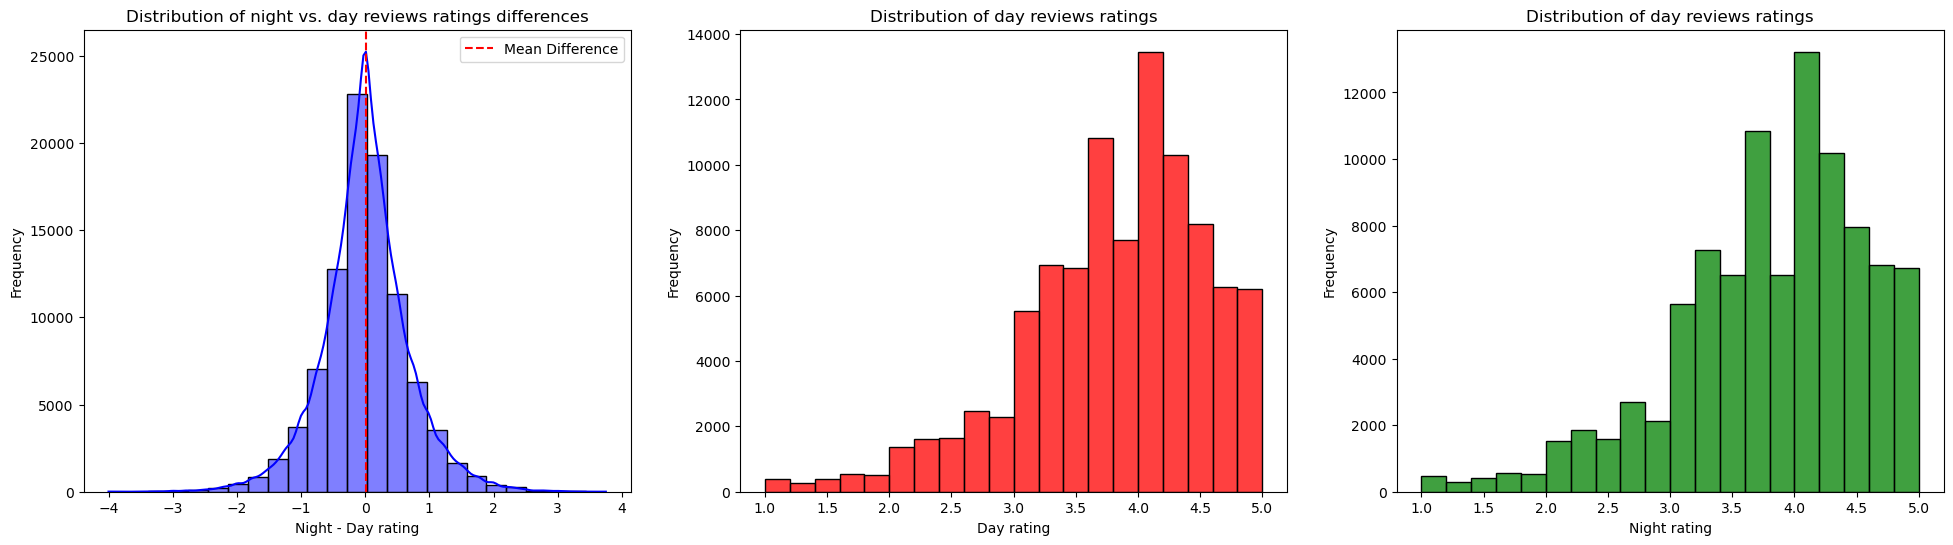
\includegraphics[width=\columnwidth]{imgs/query_5.png}
    \caption{Distribution of night vs. day reviews ratings differences}
    \label{fig:query_5}
\end{figure}

\bigskip

The distribution of reviews is stable across day and night. The mean difference is $0$: this means that the majority of users give similar ratings during day and night. However, a part of users seems to be stricter during night because bars below $0$ are higher than the symmetric ones (w.r.t $x = 0$). A deeper statistical analysis could determine if these patterns are meaningful or coincidental.

\section{Query 6: friends have similar ratings?}
This query was designed to examine the similarity in rating behaviours among friends by focusing on businesses they have both reviewed. Such similarity was quantified in terms of difference between average review stars.

As done in the previous queries, I proceeded in two steps. In the first one, all relevant documents were shaped and retrieved:
\begin{itemize}
    \item \texttt{avg\_rating}: for each \texttt{user\_id} and \texttt{business\_id}, average star rating was computed. 

\bigskip

\begin{lstlisting}[style = mongodb]
db["businesses_merged"].aggregate([{
        "$unwind" : "$reviews"
    },
    {
        "$group" : {
            "_id" : {
                "user_id" : "$reviews.user_id",
                "business_id" : "$business_id"
            },
            "avg_rating" : {
                "$avg" : "$reviews.stars"
            }
        }
    },
    {
        "$match" : {
            "avg_rating" : {
                "$ne" : None
            }
        }
    },
    {
        "$project" : {
            "_id" : 0,
            "user_id" : "$_id.user_id",
            "business_id" : "$_id.business_id",
            "avg_rating" : 1
        }
    }
])
\end{lstlisting}

\bigskip

\item \texttt{common\_ratings}: for each \texttt{user\_id} and \texttt{user\_id} of friends, \texttt{business\_id} of common reviewed businesses were found. 

\bigskip

\begin{lstlisting}[style = mongodb]
db["users_merged"].aggregate([{
        "$project" : {
            "user_id" : 1,
            "reviews" : "$reviews.business_id",
            "friends" : 1
        }
    },
    {
        "$lookup" : {
            "from" : "users_merged",
            "localField" : "friends",
            "foreignField" : "user_id",
            "pipeline" : [{
                "$project" : {
                    "user_id" : 1,
                    "reviews" : "$reviews.business_id"
                }
            }],
            "as" : "friend_reviews"
        }
    },
    {
        "$project" : {
            "friends" : 0
        }
    },
    {
        "$addFields" : {
            "shared_reviews" : {
                "$map" : {
                    "input" : "$friend_reviews",
                    "as" : "f_r",
                    "in" : {
                        "friend_id" : "$$f_r.user_id",
                        "businesses" : {
                            "$setIntersection" : ["$reviews", "$$f_r.reviews"]
                        }
                    }
                }
            }
        }
    },
    {
        "$project" : {
            "reviews" : 0,
            "friend_reviews" : 0
        }
    },
    {
        "$addFields" : {
            "shared_reviews" : {
                "$filter" : {
                    "input" : "$shared_reviews",
                    "as" : "s_r",
                    "cond" : {
                        "$gt": [{"$size": "$$s_r.businesses"}, 0]
                    }
                }
            }
        }
    },
    {
        "$unwind" : "$shared_reviews"
    },
    {
        "$project": {
            "_id" : 0,
            "user_id" : 1,
            "shared_reviews" : 1
        }
    }
])
\end{lstlisting}

\bigskip

To better understand the reasoning behind this query, the structure of the documents is presented step by step:
\begin{itemize}
    \item \texttt{\$project}: \texttt{user\_id field}, \texttt{business\_id} from the reviews array and \texttt{friends} are preserved.

\begin{lstlisting}[language=json]
{
    "user_id": "string",
    "reviews": ["business_id1", "business_id2", ...],
    "friends": ["friend_id1", "friend_id2", ...]
}
\end{lstlisting}

\item \texttt{\$lookup}: self-join operation with the \texttt{users\_merged} collection on \texttt{friends} array and \texttt{user\_ids}. The document is expanded into:

\begin{lstlisting}[language=json]
{
    "user_id": "string",
    "reviews": ["business_id1", "business_id2", ...],
    "friends": ["friend_id1", "friend_id2", ...],
    "friend_reviews": [
        {
            "user_id": "friend_id1",
            "reviews": ["business_id1", "business_id3", ...]
        },
        ...
    ]
}
\end{lstlisting}

\item \texttt{\$project}: now-redundant \texttt{friends} array is removed.

\item \texttt{\$addFields}: with \texttt{\$map} operator, the intersection of reviewed businesses between the user and each friend was computed.

\begin{lstlisting}[language=json]
{
    "user_id": "string",
    "reviews": ["business_id1", "business_id2", ...],
    "friend_reviews": [...],
    "shared_reviews": [
        {
            "friend_id": "friend_id1",
            "businesses": ["shared_business_id1", ...]
        },
        ...
    ]
}
\end{lstlisting}

\item \texttt{\$project}: \texttt{reviews} and \texttt{friend\_reviews} arrays are removed.

\item \texttt{\$addFields}: with \texttt{\$filter} entries where users share no common reviews are removed. Structure is same as previous.

\item \texttt{\$unwind}: a single user-friend relationship is now represented in a document.

\begin{lstlisting}[language=json]
{
    "user_id": "string",
    "shared_reviews": {
        "friend_id": "friend_id1",
        "businesses": ["shared_business_id1", "shared_business_id2", ...]
    }
}
\end{lstlisting}

\item \texttt{\$project}: \texttt{\_id} field is removed, resulting in the following:

\begin{lstlisting}[language=json]
{
    "user_id": "string",
    "shared_reviews": {
        "friend_id": "friend_id1",
        "businesses": ["shared_business_id1", "shared_business_id2", ...]
    }
}
\end{lstlisting}
\end{itemize}

\bigskip

\item In the second stage of the query, I combined the results collected before. Because DataFrame indexing is slow, I transformed \texttt{avg\_rating} in a dict of dicts:

\bigskip 

\begin{minted}{python}
avg_rating.reset_index()\
          .groupby("user_id")\
          .apply(lambda g: dict(zip(g["business_id"], g["avg_rating"])))\
          .to_dict()
\end{minted}

\bigskip

Then, for each document in \texttt{common\_reviewed}, I retrieved ratings for both the user and one of his / her friend (there could be more than one commonly reviewed businesses) and their averages were computed: 

\bigskip 

\begin{minted}{python}
result = []

for doc in common_reviewed:
    user_id = doc["user_id"]
    friend_id = doc["shared_reviews"]["friend_id"]
    businesses = doc["shared_reviews"]["businesses"]
    
    avg_user_ratings = [avg_rating_dict[user_id][b] for b in businesses]
    avg_friend_ratings = [avg_rating_dict[user_id][b] for b in businesses]
    
    result.append({
        "user_id" : user_id,
        "friend_id" : friend_id,
        "avg_rating_user" : pd.Series(avg_user_ratings).mean(),
        "avg_rating_friend" : pd.Series(avg_friend_ratings).mean()
    })
    
result_df = pd.DataFrame(result)
result_df
\end{minted}

\bigskip

\end{itemize}

The following histogram shows the results:

\bigskip

\begin{figure}[H]
    \centering
    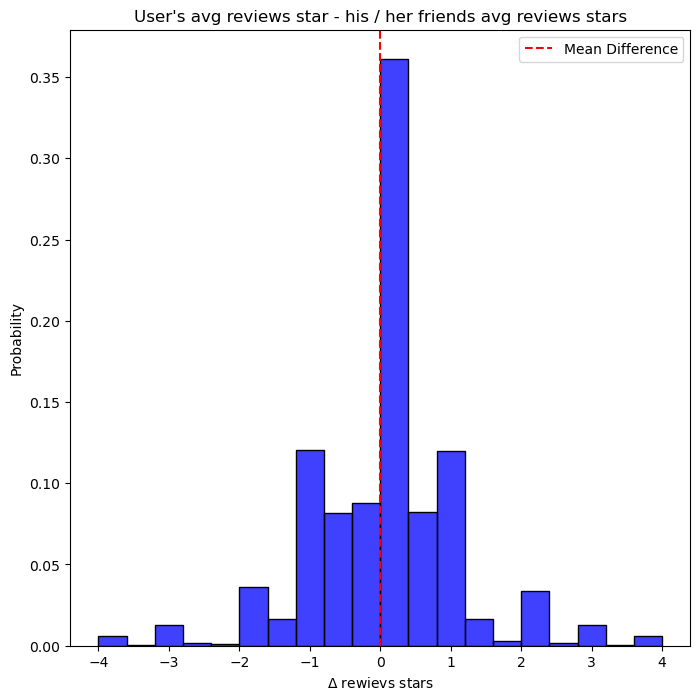
\includegraphics[width=2\columnwidth / 3]{imgs/query_6.png}
    \caption{User's average reviews star - his / her friends average reviews stars}
    \label{fig:query_6}
\end{figure}

\bigskip

The distribution is centered around zero, which suggests that users and their friends tend to give similar ratings: with probability of $0.35$, the $\Delta$ it's exactly in $0$-bin and if we consider $-1$ to $1$ bins, about $0.75$ of total friend pairs are covered. There are, however, a few cases where the differences in ratings are more extreme, ranging from $-4$ to $+4$ (users either rated a business significantly higher or lower than their friends). Despite these deviations, the red dashed line, representing the mean difference, lies at zero. 

\section{Query 7: yearly growth rate of businesses}
The growth rate of a business is defined as $g_{B, i}=\frac{n_{B, i + 1} - n_{B, i}}{n_{B, i}}$ where $n_{B, i}$ is the number of check-ins for business $B$ in year $i$. The objective of this query was to compute the growth rate of all businesses such that $\exists i, j \in [\texttt{start\_date}, \texttt{end\_date}] \,\, | \,\, i < j \land \forall k \in [i, j] \,\, | \,\, n_{B, k} > 0$ with \texttt{start\_date} and \texttt{end\_date} query parameters.

\bigskip

\begin{lstlisting}[style = mongodb]
db["businesses_merged"].aggregate([{
        "$unwind" : "$checkins"
    },
    {
        "$addFields" : {
            "year_checkin" : {
                "$year" : "$checkins"
            }
        }
    },
    {
        "$match" : {
            "$and" : [{"year_checkin" : {"$gte" : start}}, 
                    {"year_checkin" : {"$lte" : end}}]
        }
    },
    {
        "$group" : {
            "_id" : {
                "name" : "$name",
                "city" : "$city",
                "year" : "$year_checkin"
            },
            "num_checkins" : {
                "$sum" : 1
            }
        }
    },
    {
        "$sort" : {
            "_id.name" : 1,
            "_id.city" : 1,
            "_id.year" : 1
        }
    },
    {
        "$group" : {
            "_id" : {
                "name" : "$_id.name",
                "city" : "$_id.city"
            },
            "checkins_sequence" : {
                "$push" : {
                    "year" : "$_id.year",
                    "num_checkins" : "$num_checkins"
                }
            }
        }
    },
    {
        "$project" : {
            "_id" : 0,
            "name" : "$_id.name",
            "city" : "$_id.city",
            "checkins_sequence" : 1
        }
    }
])    
\end{lstlisting}

\bigskip

There were businesses with $n_{B, i} = 0$ and $n_{B, i - 1} \neq 0 \,\,\land \,\, n_{B, i + 1} \neq 0$, so the results of this query had to be filtered and the growth had to be computed. The Python code is available under \texttt{Query 7} subsection of \texttt{Queries} notebook. In particular, note the \texttt{calculate\_and\_filter\_trend} method that takes in input a \texttt{lambda} function \texttt{filter} to specify conditions on growth rate.

For the business with the longest sequence of registered check-ins, both $n_{B, i}$ and $g_{B, i}$ were plotted:

\bigskip

\begin{figure}[H]
    \centering
    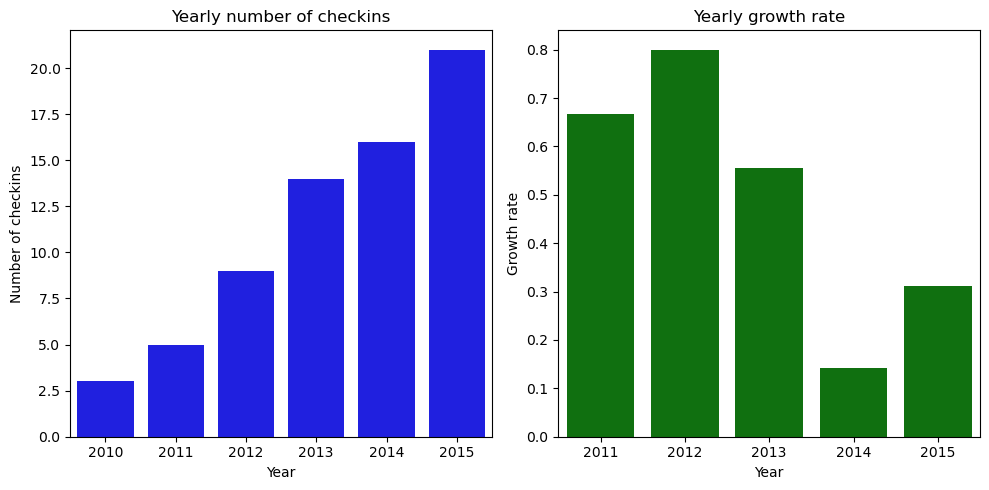
\includegraphics[width=\columnwidth]{imgs/query_7.png}
    \caption{Check-ins and yearly growth rate sequence for the selected business}
    \label{fig:query_7}
\end{figure}

\bigskip

\section{Query 8: cities with lowest sentiment for each category}
For each category, the cities with the lowest sentiment for that category were determined. To have a less biased result, only categories with sufficient number of positive and negative reviews (at least $50$ for each one) were considered.

\bigskip

\begin{lstlisting}[style = mongodb]
db["businesses_merged"].aggregate([{
        "$unwind": "$reviews"
    },
    {
        "$unwind" : "$categories" 
    },
    {
        "$group" : {
            "_id" : {
                "city" : "$city",
                "category": "$categories"
            },
            "num_positive_reviews" : {
                "$sum" : {
                    "$cond" : [{"$eq" : ["$reviews.sentiment", "positive"]}, 1, 0]
                }
            },
            "num_negative_reviews" : {
                "$sum" : {
                    "$cond" : [{"$eq" : ["$reviews.sentiment", "negative"]}, 1, 0]
                }
            }
        }
    },
    {
        "$match" : {
            "num_positive_reviews" : {
                "$gte": 50
            },
            "num_negative_reviews" : {
                "$gte" : 50
            }
        }
    },
    {
        "$addFields" : {
            "neg_to_pos_ratio" : {
                "$divide" : ["$num_negative_reviews", "$num_positive_reviews"]
            }
        }
    },
    {
        "$sort" : {
            "city" : 1,
            "name" : 1,
            "neg_to_pos_ratio" : -1
        }
    },
    {
        "$project" : {
            "_id" : 0,
            "city" : "$_id.city",
            "category" : "$_id.category",
            "tot_reviews" : {
                "$sum" : ["$num_positive_reviews", "$num_negative_reviews"]
            },
            "num_negative_reviews" : 1,
            "num_positive_reviews" : 1,
            "neg_to_pos_ratio" : 1
        }
    }
    
])    
\end{lstlisting}

\bigskip

Upon having all documents, using Pandas, widespread categories (i.e. categories in resulting DataFrame present in more than $15$ lines) were computed and for the top $3$ an histogram was plotted: 

\bigskip

\begin{figure}[H]
    \centering
    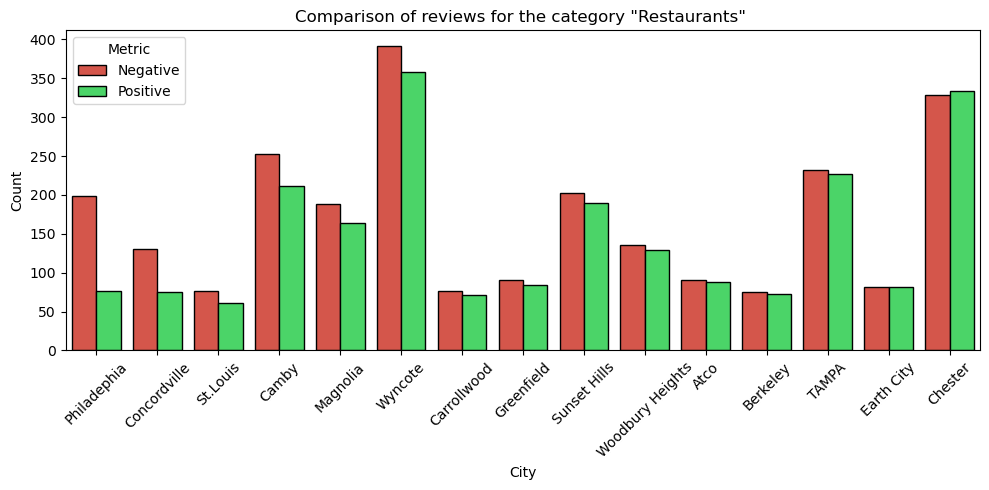
\includegraphics[width=\columnwidth]{imgs/query_8a.png}
    \caption{Comparison of reviews sentiment for the category "Restaurants"}
    \label{fig:query_8a}
\end{figure}

\bigskip

\begin{figure}[H]
    \centering
    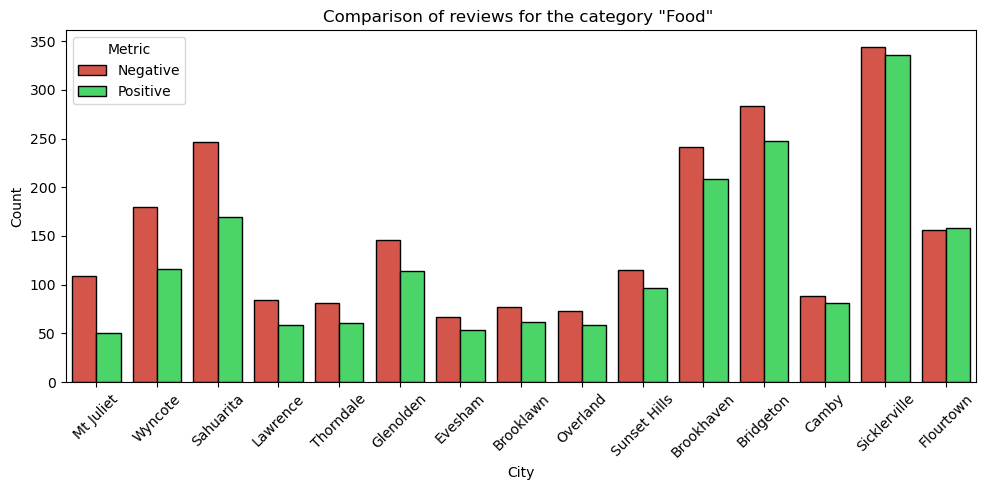
\includegraphics[width=\columnwidth ]{imgs/query_8b.png}
    \caption{Comparison of reviews sentiment for the category "Food"}
    \label{fig:query_8b}
\end{figure}

\bigskip

\begin{figure}[H]
    \centering
    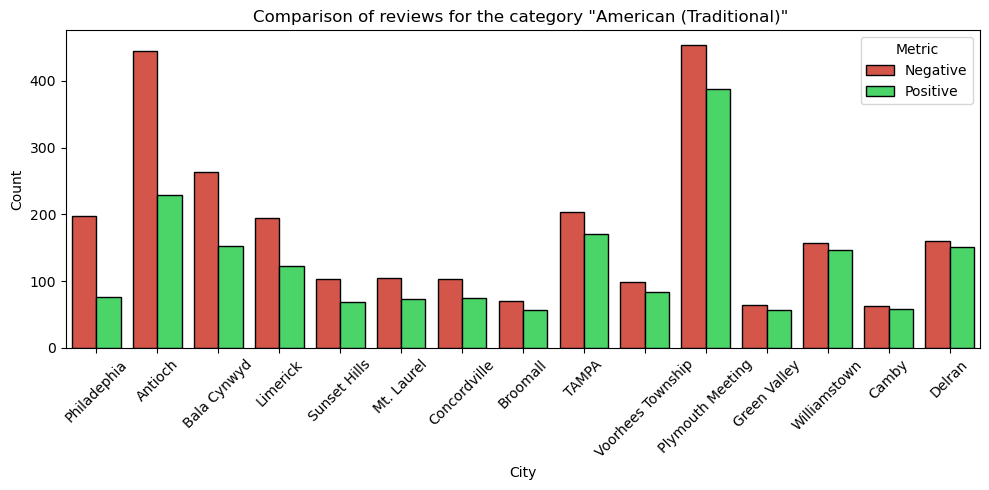
\includegraphics[width=\columnwidth]{imgs/query_8c.png}
    \caption{Comparison of reviews sentiment for the category "American (traditional)"}
    \label{fig:query_8c}
\end{figure}

\bigskip

For all categories, the sentiment distribution varies significantly between cities. Some cities show a clear dominance of negative reviews, while others have a more balanced distribution or even a higher number of positive reviews: this indicates a localized sentiment trend for lower / higher quality in certain areas.

In addition, cities with higher total reviews often have larger disparities between positive and negative sentiments, suggesting that review counts and quality perceptions may correlate, with popular locations potentially attracting more polarized opinions.

\section{Query 9: number of businesses for each bucket of possible reviews ratings}
The aim of this query was to count the number of businesses for each bucket (or bin) of possible review ratings. In particular, I defined:
$$\texttt{buckets} = [0, 0.5, ..., 4.5, 5]$$
and counted how many businesses had their average review rating in $[\texttt{buckects[i]}, \\ \texttt{buckets[i + 1]})$, using \texttt{\$bucket} operator.

\bigskip

\begin{lstlisting}[style = mongodb]
db["businesses_merged"].aggregate([{
        "$project" : {
            "business_id" : 1,
            "reviews.stars" : 1
        }
    },
    {
        "$unwind" : "$reviews"
    },
    {
        "$group" : {
            "_id" : "$business_id",
            "avg_rating" : {
                "$avg" : "$reviews.stars"
            },
            "num_reviews" : {
                "$sum" : 1
            }
        }
    },
    {
        "$match" : {
            "num_reviews" : {
                "$gte" : 25 
            }
        }
    },
    {
        "$bucket" : {
            "groupBy" : "$avg_rating",
            "boundaries" : boundaries,
            "default" : "other",
            "output" : {
                "count" : {
                    "$sum" : 1
                }
            }
        }
    },
    {
        "$densify" : {
            "field" : "_id",
            "range" : {
                "step" : step,
                "bounds" : [0.5, 5.0 + 0.5]
            }
        }
    },
    {
        "$set" : {
            "count" : {
                "$cond" : [{"$not" : ["$count"]}, 0, "$count"]
            }
        }
    },
    {
        "$project" : {
            "boundary" : "$_id", 
            "_id" : 0,
            "count" : 1
        }
    }
])
\end{lstlisting}

\bigskip

The following histogram shows the results:

\bigskip

\begin{figure}[H]
    \centering
    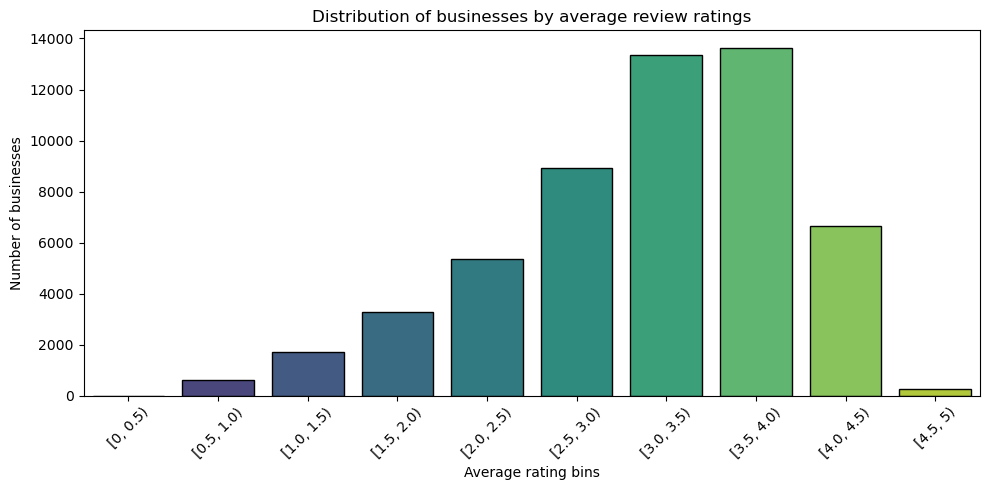
\includegraphics[width=\columnwidth]{imgs/query_9.png}
    \caption{Distribution of businesses by average review ratings}
    \label{fig:query_9}
\end{figure}

\bigskip

Most businesses have average review ratings in the range of $3.0 - 4.0$, with about $14,000$ for both $[3.0, 3.5)$ and $[3.5, 4.0)$. As ratings decrease below $3.0$ or increase above $4.0$, the number of businesses drops significantly: very few businesses have average ratings below $0.5$ or above $4.5$.

\section{Query 10: investigate the relation between sentiment and stars of reviews}
As mentioned in \ref{sent_model}, DistilBert's outputs come with a confidence measure (also called \textit{score}). 

For each star value, I counted the number of reviews with positive and negative sentiments. Then, I computed the minimum confidence $m=\min_i\,\,\text{confidence}_i$ and $M=\max_i \,\, \text{confidence}_i$ and defined:
$$\left[m, m + \frac14(M-m), m+\frac12(M-m), m+\frac34(M-m), M\right]$$
For each star and bin, I counted the number of reviews with the that number of stars and confidence in that bin.

Two steps were performed for this query:
\begin{itemize}
\item \texttt{min\_max\_confidence}: minimum and maximum confidence were computed for all reviews. 

\bigskip

\begin{lstlisting}[style = mongodb]
    db["reviews"].aggregate([{
        "$project" : {
            "_id" : 1,
            "confidence" : 1
        }
    },
    {
        "$group" : {
            "_id" : True,
            "max_confidence" : {
                "$max" : "$confidence"
            },
            "min_confidence" : {
                "$min" : "$confidence"
            }
        }
    },
    {
        "$project" : {
            "_id" : 0
        }
    }
])
\end{lstlisting}

\bigskip

\item From \texttt{min\_max\_confidence}, vector of bins was defined using Python (here not shown for the sake of shortness).

\item \texttt{query\_results}: bucket count of \texttt{confidence} was performed.

\bigskip

\begin{lstlisting}[style = mongodb]
db["reviews"].aggregate([{
        "$project" : {
            "sentiment" : 1,
            "confidence" : 1,
            "stars" : 1
        }
    },
    {
        "$group" : {
            "_id" : {
                "stars" : "$stars",
                "sentiment" : "$sentiment"
            },
            "num_reviews" : {
                "$sum" : 1
            },
            **bins_fields
        }
    },
    {
        "$project" : {
            "stars" : "$_id.stars",
            "sentiment" : "$_id.sentiment",
            "_id" : 0,
            "max_confidence" : 1,
            "min_confidence" : 1,
            "bin_1" : 1,
            "bin_2" : 1, 
            "bin_3" : 1,
            "bin_4" : 1,
            "num_reviews": 1
        }
    }
])
\end{lstlisting}

\bigskip

In particular, to avoid repeating very similar lines of code different times, I opted for dict unpacking (\texttt{**bin\_fields}) inside the \texttt{\$group} stage (the reader can look at specific code in the \texttt{Query 9} section of the \texttt{Queries} notebook).

\end{itemize}

Results were collected in the following DataFrame:

\bigskip

\begin{figure}[H]
    \centering
    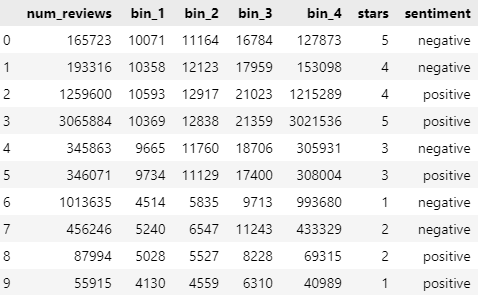
\includegraphics[width=3\columnwidth / 4]{imgs/query_10b.png}
    \caption{DataFrame of distribution of confidence score for each review star}
    \label{fig:query_10b}
\end{figure}

\bigskip

From it, two histograms were derived: 

\bigskip

\begin{figure}[H]
    \centering
    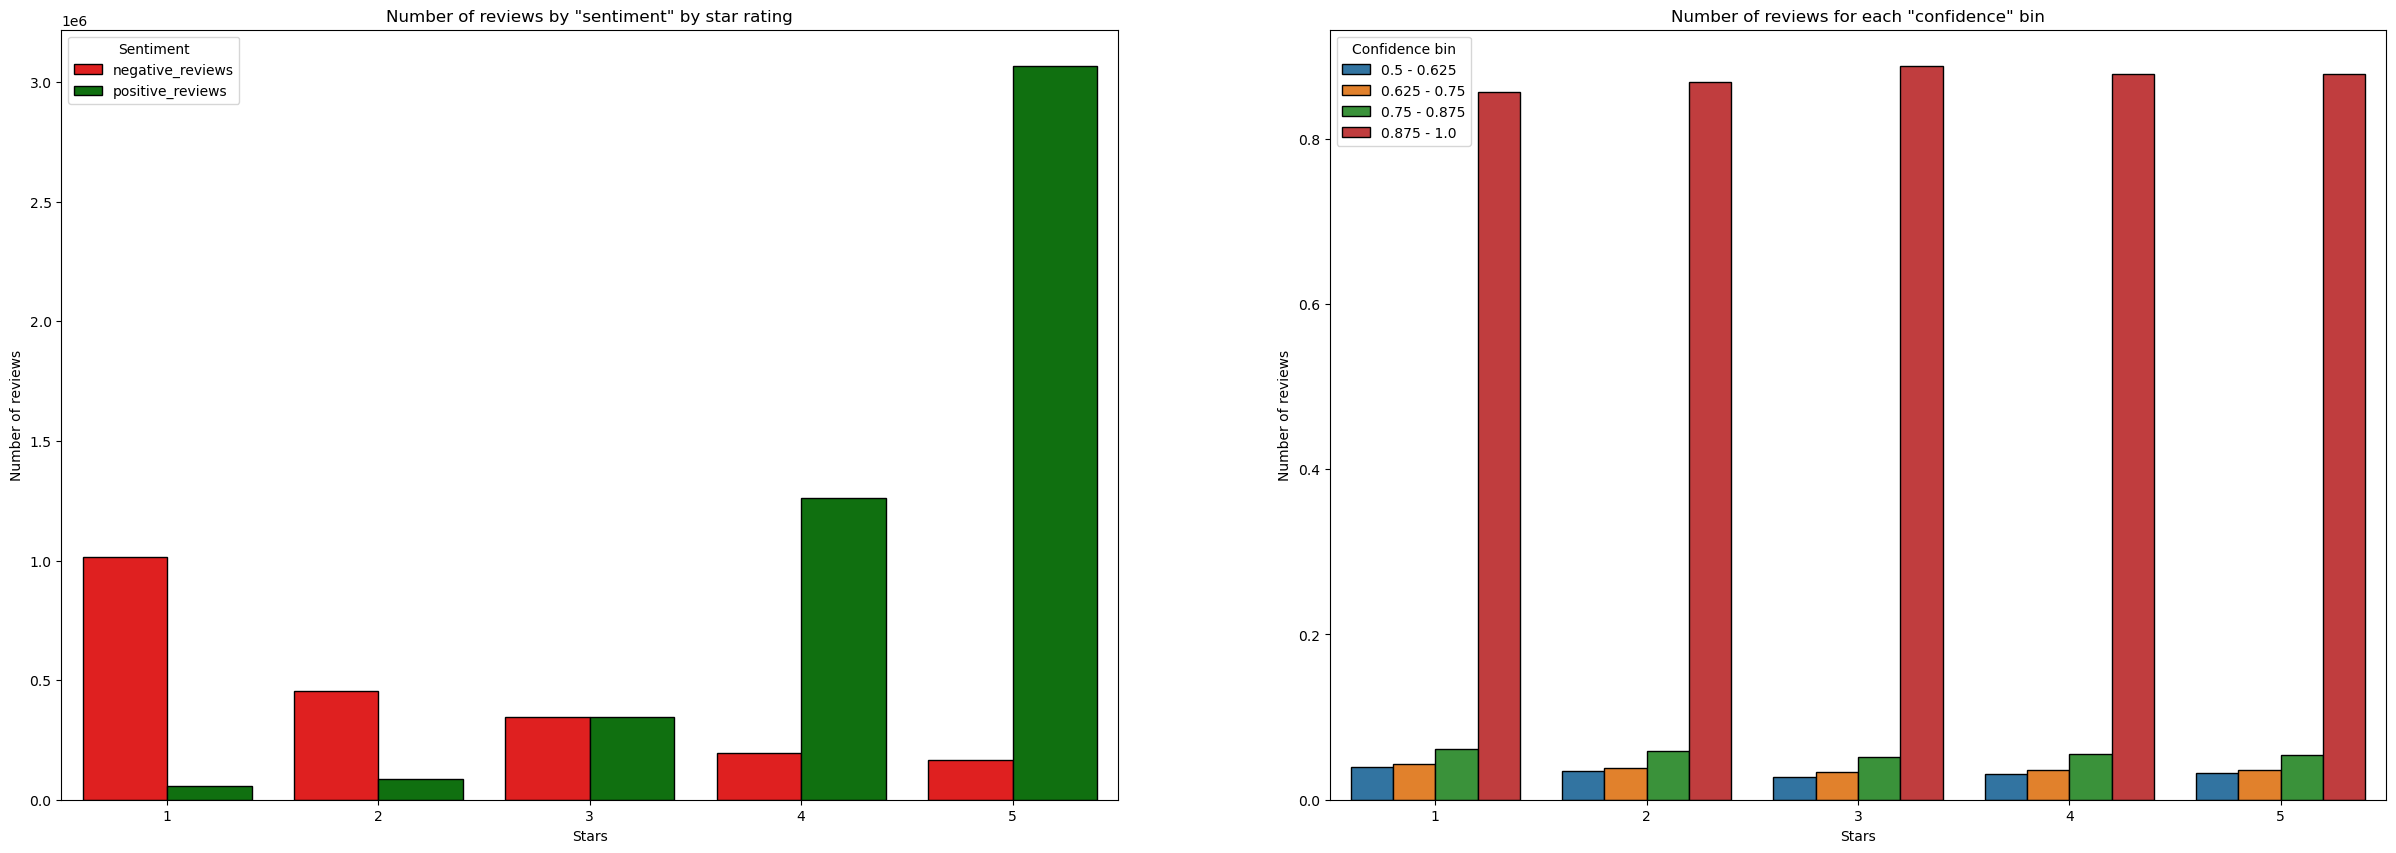
\includegraphics[width=\columnwidth]{imgs/query_10.png}
    \caption{Histogram of distribution of confidence score for each review star}
    \label{fig:query_10}
\end{figure}

\bigskip

The analysis reveals a clear relationship between sentiment and review stars. Reviews with $4$ or $5$ stars are predominantly classified as positive, while those with $1$ or $2$ stars are mostly negative, as one could intuitively think. Three-star reviews are equally classified as positive or negative: this means that I can use $3$ as threshold to discriminate outlayer reviews (see \ref{query_11}).

\section{Query 11: search for reviews outlayers}
\label{query_11}
The objective of this query was to search for reviews outlayers, i.e. reviews with positive (negative) sentiment, but low (high) number of stars under the assumption that positive (negative) sentiments are typically associated with $\text{stars} \geq 3.0$ ($\text{stars} \leq 2.0$). Moreover, the impact of this outlayers on the average reviews score was estimated. 

To guarantee low bias in the analysis, only businesses with at least 50 reviews were considered.

\bigskip

\begin{lstlisting}[style = mongodb]
db["businesses_merged"].aggregate([{
        "$match" : {
            "$expr" : {
                "$gte" : [{"$size" : "$reviews"}, 50]
            }
        }
    },
    {
        "$unwind" : "$reviews"
    },
    {
        "$group" : {
            "_id" : "$business_id",
            "name" : {
                "$first" : "$name"
            },
            "city" : {
                "$first" : "$city"
            },
            "measured_avg_rating" : {
                "$avg" : "$reviews.stars"
            },
            "measured_var_rating" : {
                "$stdDevPop" : "$reviews.stars"
            },
            "reviews" : {
                "$addToSet" : "$reviews"
            },
            "num_reviews" : {
                "$sum" : 1
            }
        }
    },
    {
        "$unwind" : "$reviews"
    },
    {
        "$match" : {
            "$expr" : {
                "$or" : [
                    {
                        "$and" : [{
                            "$gte" : ["$reviews.stars", 4]
                        }, 
                        {
                            "$eq" : ["$reviews.sentiment", "positive"]
                        }]
                    },
                    {
                        "$and" : [{
                            "$lte" : ["$reviews.stars", 2]
                        },
                        {
                            "$eq" : ["$reviews.sentiment", "negative"]
                        }]
                    }
                ]
            }
        }
    },
    {
        "$group" : {
            "_id" : "$_id",
            "name" : {
                "$first" : "$name"
            },
            "city" : {
                "$first" : "$city"
            },
            "measured_avg_rating" : {
                "$first" : "$measured_avg_rating"
            },
            "measured_var_rating" : {
                "$first" : "$measured_var_rating"
            },
            "num_reviews" : {
                "$first" : "$num_reviews"
            },
            "filtered_avg_rating" : {
                "$avg" : "$reviews.stars"
            },
            "filtered_var_rating" : {
                "$stdDevPop" : "$reviews.stars"
            },
            "num_filtered_reviews" : {
                "$sum" : 1
            }
        }
    },
    {
        "$addFields" : {
            "abs_avg_diff" : {
                "$abs" : {
                    "$subtract" : ["$filtered_avg_rating", "$measured_avg_rating"]
                }
            },
            "abs_var_diff" : {
                "$abs" : {
                    "$subtract" : ["$filtered_var_rating", "$measured_var_rating"]
                }
            },
            "biased_ratio" : {
                "$divide" : [{"$subtract" : ["$num_reviews", "$num_filtered_reviews"]}, "$num_reviews"]
            }
        }
    },
    {
        "$sort" : {
            "biased_ratio" : -1,
            "abs_var_diff" : -1,
            "abs_avg_diff" : -1
        }
    },
    {
        "$project" : {
            "business_id" : "$_id",
            "_id" : 0,
            "name" : 1,
            "city" : 1,
            "measured_avg_rating" : 1,
            "filtered_avg_rating" : 1,
            "measured_var_rating" : 1,
            "filtered_var_rating" : 1,
            "biased_ratio" : 1
        }
    }
])    
\end{lstlisting}

\bigskip

Results were collected in the following DataFrame:

\bigskip

\begin{figure}[H]
    \centering
    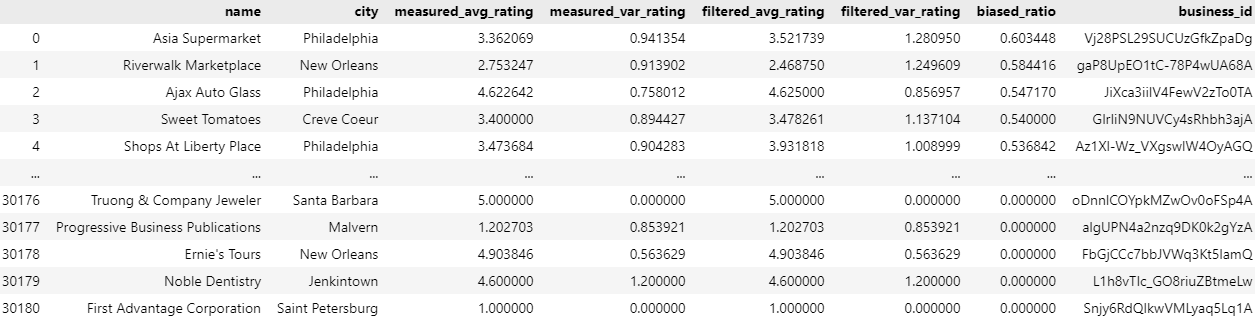
\includegraphics[width=\columnwidth]{imgs/query_11b.png}
    \caption{DataFrame of measured vs filtered average /variance rating stars}
    \label{fig:query_11b}
\end{figure}

\bigskip

From it, two bar plots representing the differences between measured and filtered average / variance of reviews stars were derived: 

\bigskip

\begin{figure}[H]
    \centering
    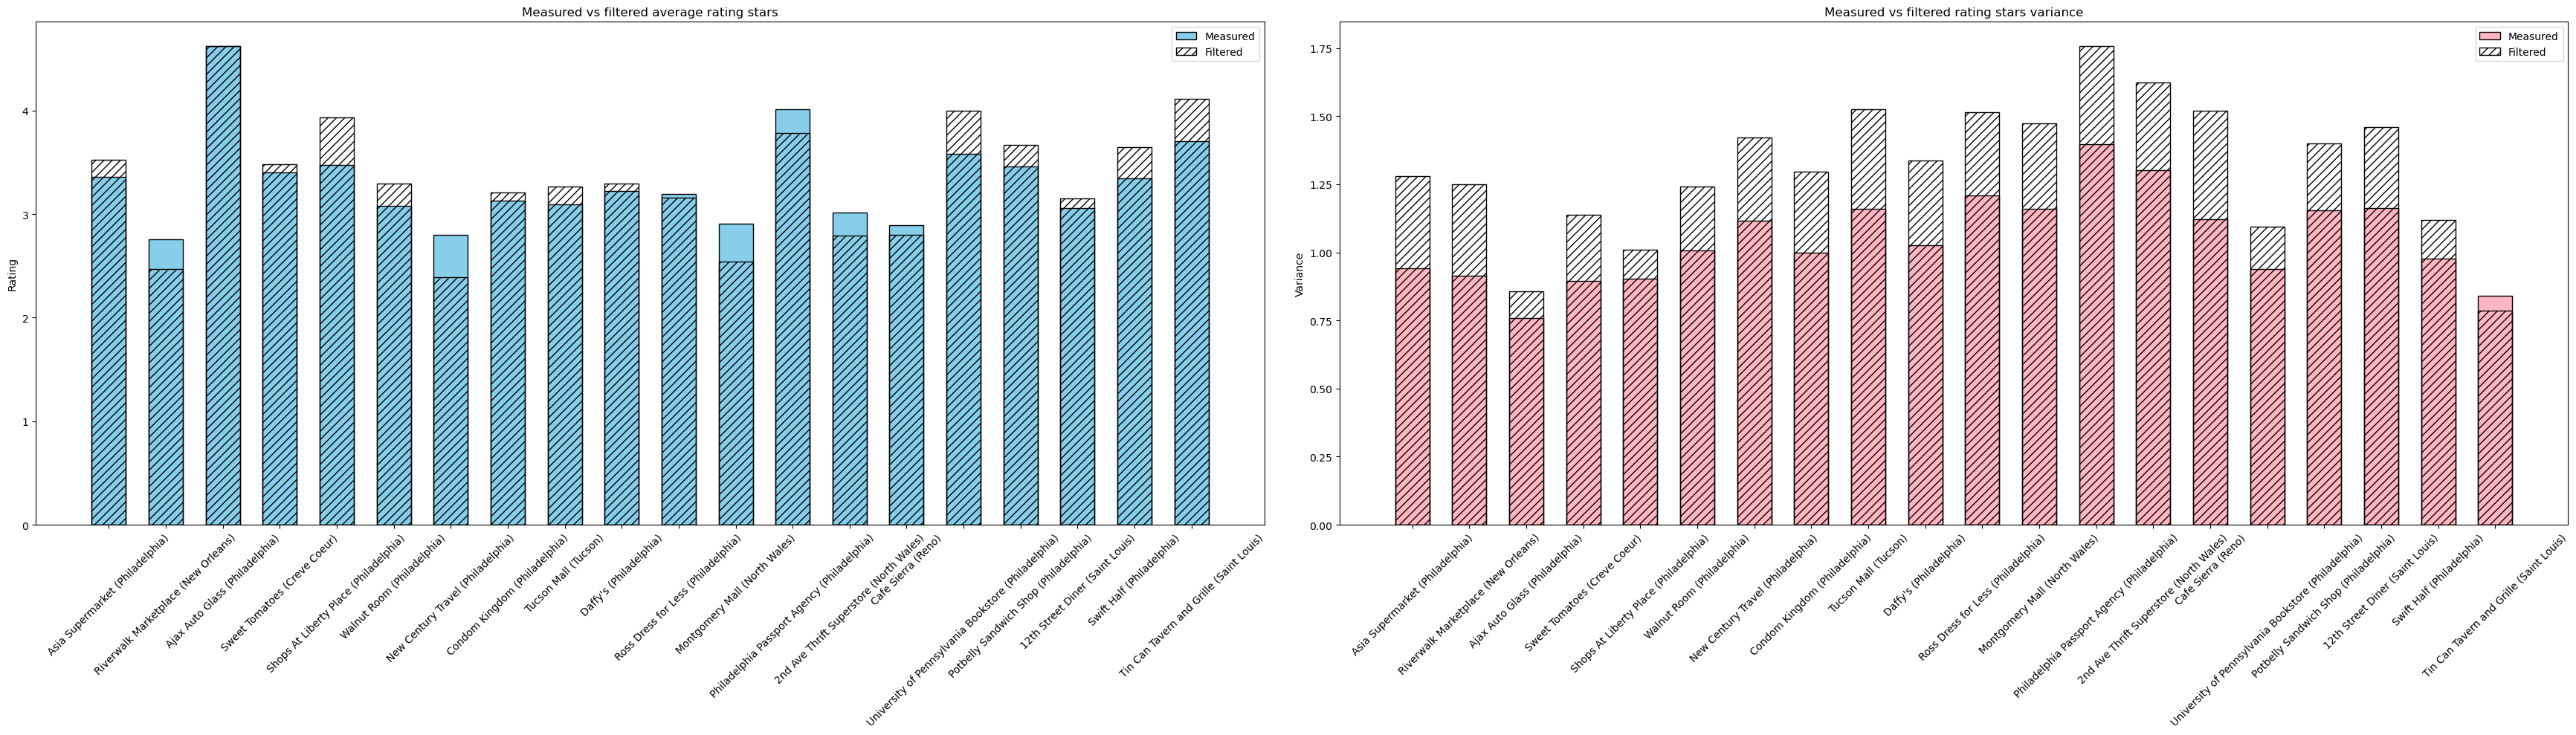
\includegraphics[width=\columnwidth]{imgs/query_11.png}
    \caption{Histograms of measured vs filtered average / variance rating stars}
    \label{fig:query_11}
\end{figure}

\bigskip

For many businesses, the filtering process slightly increased the average rating: this mean that outliers often skew ratings downward. Some other cases display minimal impact. Variance decreased significantly in most cases after excluding outliers because this review contribute to greater inconsistency in perceived business quality. 

The conclusion is that identifying and accounting for sentiment-star discrepancies can improve the reliability of aggregated ratings and better reflect actual customer experiences.

% LIST OF FIGURES
\listoffigures

% LIST OF TABLES
\listoftables

\end{document}